% =====================================================================
%  CLOSURE / ZUERICH
%  A Runtime for Non-Convergent Social Deliberation:
%  Formal Specification of a Research Instrument
%
%  Self-contained. Every object is a finite weighted graph, a bounded
%  convex program, or a construction on one. All primitives are derived
%  from stated axioms; only standard, externally published literature
%  is cited.
% =====================================================================
\documentclass[11pt,a4paper]{article}

\usepackage[utf8]{inputenc}
\usepackage[T1]{fontenc}
\usepackage{lmodern}
\usepackage[a4paper,margin=2.5cm]{geometry}
\usepackage{amsmath,amssymb,amsthm,mathtools}
\usepackage{bm}
\usepackage{booktabs,array,multirow}
\usepackage{enumitem}
\usepackage{microtype}
\usepackage{xcolor}
\usepackage{graphicx}
\usepackage{float}
\usepackage{listings}
\usepackage{algorithm}
\usepackage{algpseudocode}
\usepackage[round,sort&compress]{natbib}
\usepackage[colorlinks=true,linkcolor=blue!45!black,
            citecolor=blue!45!black,urlcolor=blue!45!black]{hyperref}
\usepackage[nameinlink,capitalise]{cleveref}

% ---------- theorem environments ----------
\newtheoremstyle{clstyle}{\topsep}{\topsep}{\itshape}{}{\bfseries}{.}{.5em}{}
\theoremstyle{clstyle}
\newtheorem{theorem}{Theorem}[section]
\newtheorem{lemma}[theorem]{Lemma}
\newtheorem{proposition}[theorem]{Proposition}
\newtheorem{corollary}[theorem]{Corollary}

\theoremstyle{definition}
\newtheorem{definition}[theorem]{Definition}
\newtheorem{construction}[theorem]{Construction}
\newtheorem{example}[theorem]{Example}
\newtheorem{axiom}{Axiom}
\newtheorem{binv}{Invariant}

\theoremstyle{remark}
\newtheorem{remark}[theorem]{Remark}
\newtheorem{notation}[theorem]{Notation}

\crefname{axiom}{Axiom}{Axioms}
\Crefname{axiom}{Axiom}{Axioms}
\crefname{binv}{Invariant}{Invariants}
\Crefname{binv}{Invariant}{Invariants}

% ---------- operators ----------
\DeclareMathOperator{\wt}{w}
\DeclareMathOperator{\cut}{cut}
\DeclareMathOperator{\Res}{Res}
\DeclareMathOperator{\Reach}{Reach}
\DeclareMathOperator{\Cl}{Cl}
\DeclareMathOperator{\dom}{dom}
\DeclareMathOperator{\Var}{Var}
\DeclareMathOperator{\dep}{depth}

% ---------- symbols ----------
\newcommand{\R}{\mathbb{R}}
\newcommand{\N}{\mathbb{N}}
\newcommand{\Gph}{\mathcal{G}}
\newcommand{\V}{V}
\newcommand{\E}{E}
\newcommand{\flo}{\beta}
\newcommand{\Cell}{\mathsf{C}}
\newcommand{\Ag}{\mathsf{A}}
\newcommand{\Sig}{\Sigma}
\newcommand{\Mod}{\mathfrak{M}}
\newcommand{\Char}{\chi}
\newcommand{\rec}{m}
\newcommand{\price}{p^{\star}}
\newcommand{\att}{\alpha}
\newcommand{\Scene}{\mathsf{S}}
\newcommand{\scenes}{\mathcal{S}}
\newcommand{\Ord}{R}
\newcommand{\Kc}{K_{c}}
\newcommand{\Vals}{\mathcal{X}}
\newcommand{\Chunks}{\mathcal{K}}
\newcommand{\Node}{n}
\newcommand{\Nodes}{\mathcal{N}}
\newcommand{\dem}{\delta}
\newcommand{\colA}{\mathsf{A}}
\newcommand{\colB}{\mathsf{B}}
\newcommand{\abs}[1]{\lvert#1\rvert}
\newcommand{\norm}[1]{\lVert#1\rVert}
\newcommand{\seekop}{\mathbf{seek}}
\newcommand{\excl}{\mathbf{excluding}}
\newcommand{\via}{\mathbf{via}}
\newcommand{\untilop}{\mathbf{until}}

\lstdefinelanguage{clo}{
  morekeywords={substrate,receivers,observable,events,floor,catalyst,
    independent,let,seek,excluding,via,until,closure,report,resolved,
    decline,record,module,prune,scene,budget},
  sensitive=true,
  morecomment=[l]{\#},
  morestring=[b]",
}
\lstdefinestyle{clostyle}{
  language=clo,
  basicstyle=\ttfamily\small,
  keywordstyle=\color{blue!70!black}\bfseries,
  commentstyle=\color{green!45!black}\itshape,
  stringstyle=\color{red!55!black},
  frame=single,
  breaklines=true,
  columns=fullflexible,
  showstringspaces=false,
}

\title{\textbf{A Runtime for Non-Convergent Social Deliberation}\\[6pt]
\large Formal Specification of an Instrument in Which Agents Deliberate,\\
Coordinate, and Decline, and in Which No Outcome Is Adjudicated}

\author{Kundai Farai Sachikonye\\
\small Technical University of Munich\\
\small \texttt{kundai.sachikonye@tum.de}}

\date{\today}

\begin{document}
\maketitle

\begin{abstract}
\noindent
We specify a runtime in which a population of bounded agents deliberates
about proposals, coordinates without shared representations, and terminates
by \emph{exhaustion of available considerations} rather than by crossing a
confidence threshold. The specification is motivated by a class of social
facts that neither belief-based nor preference-based accounts predict: a
proposal may be widely judged feasible, be opposed by no one, and never be
adopted, with no participant experiencing a decision. We show that this
outcome is the generic one, and we build an instrument in which it can be
studied.

Every object is a finite weighted graph or a construction on one. We prove,
in order: \textbf{(i)} a \emph{floor theorem}, that separating any part of a
finite weighted graph from its complement costs at least a fixed $\flo>0$,
so individuation is quantal and never point-valued; \textbf{(ii)} a
\emph{commitment theorem}, that commitment is a closure condition on a
region, that closure is \emph{strictly stronger} than any confidence
threshold, and that closure is invariant under relabelling of the provenance
and of the truth-value of what closed it, whence correctness of belief is
not a term in the coordination law; \textbf{(iii)} an \emph{attention
theorem}, that a bounded agent facing concurrent demands in a
diminishing-returns environment divides its capacity by a water-filling rule
at a single shadow price, so that an agent is present-but-preoccupied in
every context simultaneously, and that an agent which ever reflects is
unresponsive on a positive fraction of instants; \textbf{(iv)} a
\emph{coordination theorem}, that agents with disjoint internal structure
attain shared outcomes, that coordination cost vanishes exactly at
phase-lock, and that lock is achieved only above a critical coupling
$\Kc=O(\Delta\omega)$ fixed by the heterogeneity of the population, below
which the incoherent state is stable; \textbf{(v)} a \emph{composition
theorem}, that considerations compose multiplicatively with diminishing
returns, that repetition saturates strictly below completion, and that a
grounded argument requires a directed support cycle of length at least three,
so that no linear chain and no repeated single item can ground anything.

We then give the instrument. Agents are pairs of a causal knowledge graph and
a generative renderer; we prove the pair is required, since a deterministic
component alone is invariant-only and cannot distinguish an individual from a
faithful copy, while a generative component alone carries neither invariant
nor record. Population is represented as \emph{modules} --- coarse
thought-pattern regions --- and individuals are produced by pruning modules
against a demographic substrate, which we prove is prefix-containment in a
single address space rather than a change of kind. We give a domain-specific
language whose type system rejects, at compile time, arguments lacking an
exclusion clause and arguments grounded on fewer than three mutually
independent considerations, and we prove progress, preservation, determinism
modulo substrate, termination, and a two-outcome dichotomy in which
\emph{declination is a first-class result}.

Finally we establish the instrument's principal negative results, which are
methodological rather than incidental. We prove a \emph{telescoping
obstruction}: when the strengths of constituent considerations are estimated
from the same observation sequence that determines a cascade's measured
outcome, prediction and measurement are the same algebraic expression, so
every goodness-of-fit statistic attains its degenerate value on every data
set and the test has no null. We prove an \emph{attribution separation}: a
complete deterministic trace answers what happened and cannot express what
was load-bearing, and no refinement of the trace format closes the gap. The
instrument therefore refuses to report effect attribution, and we specify the
corrected, type-averaged test that does have a null together with the
diagnostic that detects when a binding has no discriminating power.

A Python prototype realises the runtime and its six implementation
invariants. We bind it to the public record of the City of Z{\"u}rich --- 11{,}406
recorded ballot outcomes since 1933, of which 2{,}580 carry district-level
results across 275 distinct municipal questions, together with 408{,}639
demographic records across twelve districts, 1993--2025 --- and report
twenty-four preregistered validation experiments, each written to falsify the
claim it tests. Twenty-four pass. Two experiments are reported as confirmed
\emph{negative} controls: the degenerate attribution test is shown to attain
$r=1$ on data generated by a process violating the theory it purports to
confirm, and a binding is exhibited on which the composition test provably
has no power.
\end{abstract}

\noindent\textbf{Keywords:} bounded agency; closure; coordination without
common knowledge; water-filling attention; synchronisation threshold;
multiplicative composition; agent-based instrument; declination; attribution
separation; research infrastructure.

\vspace{4pt}
\tableofcontents
\vspace{6pt}
\hrule

% =====================================================================
\part*{Part I --- Motivation and Setting}
\addcontentsline{toc}{part}{Part I --- Motivation and Setting}
% =====================================================================

\section{Introduction}
\label{sec:intro}

\subsection{The phenomenon}

Consider a proposal with the following properties. It is technically sound,
and the relevant professionals will say so if asked. It is affordable, and
the relevant budget officers will say so if asked. It is opposed by no
organised interest. Surveyed citizens, presented with it, express mild
approval. And it is not adopted --- not this year, not next, not in thirty
years --- and at no point does any participant experience having decided
against it.

This is not a hypothetical. It is the ordinary condition of the large
majority of feasible proposals in any functioning polity. A city does not
build a river transport system; it does not introduce a particular course of
study; it does not reconfigure a junction that everyone agrees is poor. In
each case the absence is stable, uncontested, and unaccompanied by any
decision event.

Three standard accounts fail to predict this outcome.

The \emph{common knowledge} account
\citep{lewis1969convention,schelling1960strategy,aumann1976agreeing} grounds
coordination in an infinite hierarchy of mutual knowledge. It is an
idealisation of known severity \citep{fagin1995reasoning}, and it does not
engage the case at all: the citizens in question do not lack higher-order
knowledge of one another's attitudes; they have no attitudes to know.

The \emph{preference} account holds that non-adoption reveals a preference
against. But the survey response is mildly favourable and stable under
probing, and no elicitation recovers the supposed opposing preference.

The \emph{aggregation} account \citep{hayek1945use} holds that some mechanism
combines individual information into a collective decision. In the case
described there is no aggregator: no body ever placed the question on an
agenda, and so nothing was aggregated.

We propose that all three look in the wrong place. They look at what agents
believe or prefer. We will exhibit a coordination law in which neither
belief-content, nor its truth, nor preference appears --- and in which the
observed outcome is generic.

\subsection{The thesis}

Our thesis has two halves.

\emph{Commitment is closure.} An agent commits to an outcome when every
further consideration available to it resolves into a region it has already
reached, so that no additional inquiry could change the outcome. This is a
condition on a region of a graph, not on a proposition, and we prove it
strictly stronger than any confidence threshold
(\Cref{thm:closure-stronger}).

\emph{Closure is blind.} The condition quantifies over resolutions and
mentions nothing else. It is therefore invariant under relabelling of how a
consideration was obtained (\Cref{thm:blind}) and, a fortiori, under
substitution of a false consideration for a true one with the same resolution
(\Cref{thm:truth-blind}).

The proposal above is then explained exactly: it is believed, it is
reachable, and it never closes, because some available-but-uninvoked
consideration resolves elsewhere. And a \emph{failure of closure is not an
event} --- it is the persistence of a standing condition, which is why nobody
experiences it as a decision and why it is stable
(\Cref{rem:no-decision}).

\subsection{Why an instrument}

The phenomenon is difficult to study by conventional means. It is
constituted by a non-event, so it has no timestamp; the relevant
counterfactual (what would have closed) is not observable; and the standard
experimental manipulation --- present the proposal and measure attitude
change --- destroys the phenomenon by placing the proposal on an agenda,
which is precisely the intervention whose absence defines the case.

We therefore specify a runtime in which the phenomenon can be instantiated,
inhabited, and perturbed. A human participant enters a simulated polity, may
address any of its agents, and may attempt to bring about the adoption of a
proposal of their choosing. The agents are not scripted respondents. They
have their own purposes, their own finite attention divided across contexts
the participant never sees, their own questions, and their own capacity to
decline. They do not represent the participant's proposal as a task.

The instrument's defining property is that it \emph{adjudicates nothing}. It
has no success state, computes no score, and --- we prove --- cannot compute
one, since the quantity that would be required is not expressible in it
(\Cref{thm:no-verdict,thm:attribution}). What it produces is a complete,
interrogable record of what propagated, which the investigator interprets.

\subsection{What is proved, and in what order}

\Cref{sec:floor} derives the floor. \Cref{sec:closure} derives commitment and
its two blindness results. \Cref{sec:attention} derives water-filling
attention and phase alternation. \Cref{sec:society} derives coordination,
the synchronisation threshold, and crowd sharpening. \Cref{sec:compose}
derives multiplicative composition, saturation, and the support-cycle
condition. \Cref{sec:agent} specifies the agent as a graph--renderer pair and
proves the pair necessary. \Cref{sec:population} specifies modules,
substrate, and pruning. \Cref{sec:language} gives the language, its type
system, and its metatheory. \Cref{sec:runtime} gives the global runtime.
\Cref{sec:negative} proves the two negative results and specifies the
corrected tests. \Cref{sec:blueprint} states the implementation invariants.
\Cref{sec:validation} reports the validation suite.
\Cref{sec:ethics,sec:limits} state the ethical and formal limits.

\subsection{What is not claimed}

We do not claim that human deliberation \emph{is} a finite weighted graph or
a convex program. We claim that any system satisfying the stated axioms has
the structure derived, that the structure suffices to instantiate the
phenomenon of \Cref{sec:intro}, and that the instrument is therefore a
legitimate object of study in its own right. Whether it is a good model of
any particular human population is an empirical question we do not settle,
and \Cref{sec:limits} states precisely which of our results would survive a
negative answer.

We do not claim the instrument measures persuasion. \Cref{sec:negative}
proves it cannot.

Interpretive readings of formal objects --- ``belief,'' ``attention,''
``identity,'' ``conversation'' --- are marked as orientation and confined to
remarks. No theorem depends on them.

% =====================================================================
\section{Primitives and axioms}
\label{sec:axioms}
% =====================================================================

\begin{definition}[Contact graph]
\label{def:contact}
A \emph{contact graph} is a triple $\Gph=(\V,\E,\wt)$ with $\V$ a finite
nonempty vertex set, $\E\subseteq\binom{\V}{2}$, and
$\wt:\E\to\R_{>0}$. We assume $\Gph$ connected. Vertices are
\emph{positions}; an edge $uv$ records that $u$ and $v$ are \emph{in
contact}, and $\wt(uv)$ is the cost of telling them apart.
\end{definition}

\begin{definition}[Cut; separation cost]
\label{def:cut}
For $\varnothing\neq A\subsetneq\V$,
$\cut(A)=\{uv\in\E: u\in A,\ v\in\V\setminus A\}$ with
$\wt(\cut(A))=\sum_{e\in\cut(A)}\wt(e)$, and
$\Res(\Gph)=\min_{\varnothing\neq A\subsetneq\V}\wt(\cut(A))$.
\end{definition}

We state six axioms. The first five constrain the agent and may be honoured
by construction in a synthetic one. The sixth constrains the
\emph{environment} and is marked throughout wherever it is used.

\begin{axiom}[Finiteness]
\label{ax:finite}
Every graph is finite, and every agent's set of concurrent contexts is
finite.
\end{axiom}

\begin{axiom}[Presence]
\label{ax:present}
At every instant an agent occupies exactly one position; its graph is
connected and nonempty.
\end{axiom}

\begin{axiom}[Costly individuation]
\label{ax:costly}
No distinction is free: there is $\flo>0$ with $\wt(e)\ge\flo$ for all
$e\in\E$.
\end{axiom}

\begin{axiom}[Act floor and bounded capacity]
\label{ax:actfloor}
Every committed act costs at least $\flo_a>0$, and an agent has a finite
capacity $\att>0$ per unit time to divide across its contexts.
\end{axiom}

\begin{axiom}[Phase exclusion]
\label{ax:phase}
Forming a new distinction and committing an act draw on the same
instantaneous capacity and cannot co-occur: at each instant an agent is in
exactly one of a \emph{construction} phase or a \emph{commitment} phase.
\end{axiom}

\begin{axiom}[Diminishing returns --- environmental]
\label{ax:concave}
Each context's gain profile $\gamma$ is nondecreasing and concave.
\emph{This constrains the world the agent acts in, not the agent.} It is
invoked only where named.
\end{axiom}

\begin{remark}[The floor is motivated, not merely posited]
\label{rem:floor-motivated}
\Cref{ax:costly} may be argued rather than stipulated. To individuate a part
$A$ is to tell it from $\V\setminus A$. If that comparison could be
\emph{finished}, the complement would be an exhausted catalogue. An agent
always in some state (\Cref{ax:present}) whose complement is never an
exhausted catalogue leaves on each comparison an irreducible remainder;
that remainder is the floor. Similarly for \Cref{ax:actfloor}: an act of
zero cost deposits nothing and so distinguishes no before from after, and an
operation that changes nothing is not an act but a no-op that did not occur.
We take both as axioms and prove from them.
\end{remark}

\begin{proposition}[The axioms are consistent and non-vacuous]
\label{prop:consistency}
For every $n\ge2$ there is a contact graph on $n$ positions satisfying
\Cref{ax:finite,ax:present,ax:costly}, with $\flo$ arbitrary in $(0,\infty)$.
\end{proposition}

\begin{proof}
Take the path $v_1v_2\cdots v_n$ with all weights $\flo$. It is finite,
connected, nonempty, and every weight equals $\flo>0$.
\end{proof}

% =====================================================================
\part*{Part II --- The Coordination Law}
\addcontentsline{toc}{part}{Part II --- The Coordination Law}
% =====================================================================

\section{The floor}
\label{sec:floor}

\begin{theorem}[Floor]
\label{thm:floor}
Let $\Gph$ be a connected contact graph satisfying \Cref{ax:costly}. Then
$\Res(\Gph)\ge\flo>0$: no nonempty proper part can be separated from its
complement at zero cost, and the bound is independent of the part.
\end{theorem}

\begin{proof}
Let $\varnothing\neq A\subsetneq\V$. By connectedness there is at least one
edge with one endpoint in $A$ and one in $\V\setminus A$; otherwise $\Gph$
decomposes into two components. So $\cut(A)\neq\varnothing$ and
$\wt(\cut(A))=\sum_{e\in\cut(A)}\wt(e)\ge\flo\abs{\cut(A)}\ge\flo$ by
\Cref{ax:costly}. The minimum over the finitely many admissible $A$ is
attained and inherits the bound.
\end{proof}

\begin{remark}[What the floor theorem establishes]
\label{rem:floor-content}
The content is not a numerical value --- $\flo$ is whatever the least weight
happens to be --- but the \emph{absence of a limiting process}. There is no
sequence of ever-cheaper separations tending to zero. This matters because
the alternative trivialises the closure conditions below: if a part could be
individuated at arbitrarily small cost, individuating and not individuating
would differ by degree, and a binary commitment condition would have no
content. The floor is the guarantee that individuation is quantal.
\end{remark}

\begin{theorem}[Individuation is regional]
\label{thm:regional}
There exist connected contact graphs in which the minimum of \Cref{def:cut}
is attained at no singleton: for every $v\in\V$,
$\wt(\cut(\{v\}))>\Res(\Gph)$.
\end{theorem}

\begin{proof}
Let $K,K'$ be disjoint triangles with all internal weights $10$, joined by a
single edge $e^{*}$ of weight $1$. The bipartition $A=V(K)$ has
$\cut(A)=\{e^{*}\}$, cost $1$. Any singleton has at least two incident
internal edges of weight $10$, so cut cost $\ge20>1$. Hence $\Res(\Gph)=1$,
attained by the bipartition and by no singleton.
\end{proof}

\begin{corollary}[No individuation at a position]
\label{cor:no-point}
Separation is a property of the pair $(A,\V\setminus A)$, and the
interesting minima are attained at regions of positive size. One cannot in
general speak of ``the individuation at $v$.''
\end{corollary}

\begin{proof}
Immediate from \Cref{thm:regional}: the minimiser has $\abs{A}=3$ and
$\Res(\Gph)$ is the cut cost of no singleton.
\end{proof}

\begin{remark}[Individuation by negation]
\label{rem:negation}
\Cref{cor:no-point} has a reading that recurs below. What individuates $A$
is not an intrinsic feature of $A$ but the cut separating it from
$\V\setminus A$ --- what $A$ is \emph{not}. A part with no complement is not
individuated at all, which is why \Cref{def:cut} excludes $A=\varnothing$ and
$A=\V$. Every later construction inherits this two-sidedness, and it is the
formal reason the language of \Cref{sec:language} makes an exclusion clause
mandatory (\Cref{thm:exclusion}).
\end{remark}

\begin{definition}[Sufficient region]
\label{def:sufficient}
Given a tolerance $\tau>0$, a region $\Cell$ with
$\varnothing\neq\Cell\subsetneq\V$ is \emph{$\tau$-sufficient} if
$\Res(\Gph\!\restriction_{\Cell})\le\tau$, where $\Gph\!\restriction_{\Cell}$
is the induced subgraph. Write $\Sig_\tau(\Gph)$ for the set of
$\tau$-sufficient regions.
\end{definition}

\begin{remark}[Reading the definition]
\label{rem:sufficient}
A region is sufficient when its internal separations are cheap relative to
$\tau$ --- when, from outside, it may be treated as one thing. The
definition is deliberately coarse: it asks whether the region holds together
at tolerance $\tau$, not whether it is correct or well chosen.
\end{remark}

\begin{definition}[Level graph]
\label{def:level}
For a partition $\mathcal{P}=\{\Cell_1,\dots,\Cell_r\}$ of $\V$, the
\emph{level graph} $\Gph/\mathcal{P}$ has the blocks as positions, an edge
$\Cell_a\Cell_b$ whenever some edge of $\Gph$ joins them, and weight
$\wt'(\Cell_a\Cell_b)=\sum\{\wt(uv): u\in\Cell_a, v\in\Cell_b\}$.
\end{definition}

\begin{proposition}[The level graph is a contact graph]
\label{prop:level}
If $\Gph$ is a connected contact graph with constant $\flo$ and
$\mathcal{P}$ partitions $\V$, then $\Gph/\mathcal{P}$ is a connected contact
graph with the same $\flo$.
\end{proposition}

\begin{proof}
Finiteness and nonemptiness are inherited. Every edge of the quotient arises
from at least one edge of $\Gph$ and its weight is a sum of terms each
$\ge\flo$, so $\wt'\ge\flo$. For connectedness, take
$\Cell_a,\Cell_b$ and $u\in\Cell_a$, $v\in\Cell_b$; a $u$--$v$ path in
$\Gph$ maps to a walk in the quotient.
\end{proof}

\begin{theorem}[No privileged level]
\label{thm:nopriv}
Let $\mathcal{P}$ partition $\V$. Then \Cref{thm:floor,thm:regional} apply
verbatim to $\Gph/\mathcal{P}$, and the construction of
\Cref{def:sufficient} is computed there by the same formula with no
aggregation operator. Consequently a sub-question, an agent, and a
population are the same kind of object evaluated at different depths.
\end{theorem}

\begin{proof}
By \Cref{prop:level} the quotient satisfies
\Cref{ax:finite,ax:present,ax:costly}, so every theorem derived from those
axioms holds of it. \Cref{def:sufficient} refers only to induced subgraphs
and a tolerance, both defined for the quotient, and to no feature of $\V$,
of position identity, or of any other level. Iterating the quotient
construction yields contact graphs at every stage, so no stage is
distinguished.
\end{proof}

\begin{remark}[No aggregator is required, and this is the point]
\label{rem:no-agg}
One might expect passing from agents to a population to require an
aggregation operator combining the agents' values. \Cref{thm:nopriv} shows
none is needed, and the reason is structural. The population's coordinates
are not computed \emph{from} the agents'; they are computed from the
population's own structure in the level graph, by the same formula. This
matters because an aggregation operator would have to be evaluated by some
observer holding all agents' values at once, and no such observer exists in
the situations of \Cref{sec:intro}. Compare \citet{hayek1945use}: the
conclusion agrees, the mechanism differs.
\end{remark}

\begin{proposition}[Sufficiency is not inherited in either direction]
\label{prop:not-inherited}
There are contact graphs and partitions in which every block is
$\tau$-sufficient while the level graph contains a region that is not, and
conversely.
\end{proposition}

\begin{proof}
\emph{Blocks sufficient, level not}: three disjoint triangles with internal
weights $1$ (each $\Res=2$, so $\tau$-sufficient at $\tau=2$), joined
pairwise by edges of weight $100$; the level graph is a triangle with all
weights $100$ and minimum cut $200>\tau$. \emph{Level sufficient, blocks
not}: two blocks joined by an edge of weight $1$, each internally a
two-vertex path of weight $100$; each block has $\Res=100>\tau$, the level
graph has $\Res=1\le\tau$.
\end{proof}

\begin{remark}[Why \Cref{prop:not-inherited} matters]
\label{rem:not-inherited}
\Cref{thm:nopriv} says the \emph{construction} applies at every level; it
does not say properties transfer between levels. A population of
individually coherent agents may fail to cohere, and a coherent population
may contain incoherent members. Both occur, and neither is predicted by the
other.
\end{remark}

% =====================================================================
\section{Commitment, closure, and blindness}
\label{sec:closure}
% =====================================================================

We now define commitment. The definition is a condition on a region and
makes no reference to the truth or the origin of anything.

\begin{definition}[Consideration]
\label{def:catalyst}
A \emph{consideration} is a pair $\gamma=(\mathrm{src},\rho_\gamma)$ in
which $\mathrm{src}$ is an arbitrary label, the \emph{provenance}, and
$\rho_\gamma:\V\rightharpoonup\Sig_\tau(\Gph)$ is a partial map, the
\emph{resolution}, assigning to a position the sufficient region that
invoking $\gamma$ from that position reaches. Write $\dom\gamma$ for its
domain.
\end{definition}

\begin{remark}[Provenance is a label and nothing else]
\label{rem:provenance}
The provenance records where a resolution came from --- direct verification,
testimony, inference, rumour. It is deliberately an arbitrary label carrying
no structure: no operation of the theory reads it, and it enters no formula
below. We include it explicitly rather than omit it because
\Cref{thm:blind} is precisely that it may be permuted freely, and one cannot
permute what is not there.
\end{remark}

\begin{definition}[Reach; closure]
\label{def:closure}
For a seed $v_0\in\V$ and a finite set $\Gamma$ of considerations, the
\emph{reach} is
\[
\Reach(v_0,\Gamma)=\{\rho_\gamma(v_0):\gamma\in\Gamma,\ v_0\in\dom\gamma\}
\subseteq\Sig_\tau(\Gph).
\]
Given an \emph{available} set $\Gamma$ and an \emph{invoked} subset
$\Gamma'\subseteq\Gamma$, the search is \emph{closed} at $\Gamma'$ if
$\Reach(v_0,\Gamma)=\Reach(v_0,\Gamma')$ --- every available but uninvoked
consideration resolves into a region already reached. Write
$\Cl(v_0,\Gamma',\Gamma)$.
\end{definition}

\begin{definition}[Commitment]
\label{def:commitment}
An agent \emph{commits} to $\Cell$ from $v_0$ when $\Cl(v_0,\Gamma',\Gamma)$
holds and $\Cell\in\Reach(v_0,\Gamma')$.
\end{definition}

\begin{theorem}[Closure is strictly stronger than a confidence threshold]
\label{thm:closure-stronger}
There exist contact graphs, seeds, consideration sets, and thresholds
$\theta\in(0,1]$ such that the invoked considerations carry confidence at
least $\theta$ while the search is not closed: some uninvoked available
consideration resolves into a region not in $\Reach(v_0,\Gamma')$.
\end{theorem}

\begin{proof}
Let $\Gph$ be two disjoint triangles $A,B$ with all internal weights $1$,
joined by a single edge of weight $1$; it is connected and satisfies
\Cref{ax:costly} with $\flo=1$. Fix $\tau=2$, so $A$ and $B$ are each
$\tau$-sufficient. Let $v_0\in A$ and
$\Gamma=\{\gamma_A,\gamma_B\}$ with $\rho_{\gamma_A}(v_0)=A$,
$\rho_{\gamma_B}(v_0)=B$, each of confidence $1$, so any $\theta\le1$ is met
by either alone. Take $\Gamma'=\{\gamma_A\}$: the threshold is satisfied,
but $\Reach(v_0,\Gamma')=\{A\}\neq\{A,B\}=\Reach(v_0,\Gamma)$, so closure
fails.
\end{proof}

\begin{corollary}[High confidence does not entail commitment]
\label{cor:conf}
An agent may hold a belief with maximal confidence and not commit, if an
available consideration reaches a distinct region. Confidence is a property
of what has been invoked; closure is a property of what remains available.
\end{corollary}

\begin{proof}
Immediate from \Cref{thm:closure-stronger} with \Cref{def:commitment}.
\end{proof}

\begin{remark}[Availability is not determined by the graph]
\label{rem:availability}
\Cref{def:closure} quantifies over an \emph{available} set the graph does not
determine: which considerations are available is a fact about an agent's
situation, not about the structure it individuates. Closure is therefore
decidable \emph{given} $\Gamma$ (\Cref{prop:decidable}) and not decidable
from the graph alone. This is a genuine limitation and we do not disguise
it; it is also the correct placement of the difficulty, since the hard
practical question is always \emph{what else should have been considered},
and a theory answering it from structure alone would claim too much.
\end{remark}

\begin{proposition}[Closure is decidable given availability]
\label{prop:decidable}
Given finite $\Gph$, seed $v_0$, finite $\Gamma$ and $\Gamma'\subseteq\Gamma$,
$\Cl(v_0,\Gamma',\Gamma)$ is decidable in time
$O(\abs{\Gamma}T_\rho+\abs{\Gamma}^2\abs{\V})$, where $T_\rho$ bounds the
cost of one resolution.
\end{proposition}

\begin{proof}
Evaluate $\rho_\gamma(v_0)$ for each applicable $\gamma$, costing
$O(\abs{\Gamma}T_\rho)$ and yielding at most $\abs{\Gamma}$ regions. Form
both reach sets and compare, with region equality tested as subset equality
in $O(\abs{\V})$ per comparison and at most $\abs{\Gamma}^2$ comparisons.
Correctness is immediate from \Cref{def:closure}.
\end{proof}

\begin{proposition}[Monotone in what is invoked]
\label{prop:mono-invoked}
If $\Gamma'\subseteq\Gamma''\subseteq\Gamma$ and $\Cl(v_0,\Gamma',\Gamma)$
holds, then $\Cl(v_0,\Gamma'',\Gamma)$ holds.
\end{proposition}

\begin{proof}
$\Gamma'\subseteq\Gamma''$ gives
$\Reach(v_0,\Gamma')\subseteq\Reach(v_0,\Gamma'')$, and
$\Gamma''\subseteq\Gamma$ gives
$\Reach(v_0,\Gamma'')\subseteq\Reach(v_0,\Gamma)$. The outer two coincide by
hypothesis, so all three do.
\end{proof}

\begin{remark}[Not monotone in what is available]
\label{rem:not-mono-avail}
The corresponding statement for $\Gamma$ is false, and its failure is the
substance of \Cref{sec:instrument-behaviour}. Enlarging the available set can
\emph{destroy} closure: a search closed against $\Gamma$ may fail to be
closed against $\Gamma\cup\{\gamma\}$ if $\gamma$ reaches a new region. A
population that learns of a new consideration may therefore cease to be
committed to what it was committed to, without anyone having changed their
mind about anything already considered. \Cref{sec:validation} (E14) measures
how often this occurs.
\end{remark}

\subsection{Blindness}
\label{sec:blind}

\begin{definition}[Provenance relabelling]
\label{def:relabel}
A \emph{provenance relabelling} is a map $\sigma$ sending
$\gamma=(\mathrm{src},\rho_\gamma)$ to
$\sigma\gamma=(\sigma(\mathrm{src}),\rho_\gamma)$, altering the label and
leaving the resolution unchanged; it extends elementwise to sets.
\end{definition}

\begin{theorem}[Provenance-blindness]
\label{thm:blind}
For every relabelling $\sigma$, seed $v_0$, available $\Gamma$ and invoked
$\Gamma'$,
\[
\Reach(v_0,\sigma\Gamma)=\Reach(v_0,\Gamma),\qquad
\Cl(v_0,\sigma\Gamma',\sigma\Gamma)\iff\Cl(v_0,\Gamma',\Gamma).
\]
Commitment is invariant under arbitrary relabelling of provenance.
\end{theorem}

\begin{proof}
By \Cref{def:relabel}, $\rho_{\sigma\gamma}=\rho_\gamma$ and
$\dom\sigma\gamma=\dom\gamma$ for every $\gamma$. Hence
$\Reach(v_0,\sigma\Gamma)
=\{\rho_{\sigma\gamma}(v_0)\}=\{\rho_{\gamma}(v_0)\}=\Reach(v_0,\Gamma)$,
and identically for $\Gamma'$. \Cref{def:closure} is an equality of reach
sets, both unchanged, so it holds for $\sigma$-images exactly when for the
originals; \Cref{def:commitment} is defined from reach and closure alone.
\end{proof}

\begin{corollary}[Disjoint routes, identical commitment]
\label{cor:routes}
Let two agents share a seed and tolerance and let their consideration sets
have \emph{no provenance in common} but equal reach sets, and correspondingly
for their invoked subsets. Then they commit to exactly the same regions.
\end{corollary}

\begin{proof}
Commitment depends only on reach and closure (\Cref{def:commitment}), equal
by hypothesis; disjointness of provenance is irrelevant by \Cref{thm:blind}.
\end{proof}

\begin{definition}[Veridical assignment]
\label{def:veridical}
A \emph{veridical assignment} $\nu$ assigns to each consideration a region
$\nu(\gamma)\in\Sig_\tau(\Gph)$, the region that \emph{would} be reached were
the consideration correct. A consideration is \emph{veridical at} $v_0$ if
$\rho_\gamma(v_0)=\nu(\gamma)$, and \emph{false at} $v_0$ otherwise.
\end{definition}

\begin{remark}[The status of $\nu$]
\label{rem:nu}
The veridical assignment is external: nothing in the axioms determines it,
and no construction computes it. It is introduced solely in order to
\emph{state} \Cref{thm:truth-blind}, which says the closure relation does not
see it. This is the honest way to formalise a negative claim about truth:
one must name the notion in order to prove independence from it.
\end{remark}

\begin{theorem}[Truth-blindness]
\label{thm:truth-blind}
Let $\widetilde\Gamma$ be obtained from $\Gamma$ by replacing any collection
of considerations $\gamma$ by $\widetilde\gamma$ with
$\rho_{\widetilde\gamma}=\rho_\gamma$ and arbitrary veridicality. Then
$\Cl(v_0,\widetilde{\Gamma'},\widetilde\Gamma)\iff\Cl(v_0,\Gamma',\Gamma)$
and the committed regions are identical. Correctness is not a term in the
commitment condition.
\end{theorem}

\begin{proof}
By hypothesis $\rho_{\widetilde\gamma}=\rho_\gamma$ for replaced
considerations and trivially for unreplaced ones, so both reach sets are
unchanged by the computation in \Cref{thm:blind}. \Cref{def:closure} is an
equality of reach sets, hence preserved, and \Cref{def:commitment} is defined
from reach and closure. The assignment $\nu$ appears in neither definition,
so no step depends on it.
\end{proof}

\begin{remark}[Scope of \Cref{thm:truth-blind}]
\label{rem:truth-scope}
This is the central claim and is easily overread.

\emph{Asserted}: the condition determining whether commitment occurs is
independent of the veridicality of what produces it. Two populations
identical in resolutions and differing arbitrarily in truth commit
identically.

\emph{Not asserted}: that truth is unimportant, or that a population running
on false considerations fares as well as one running on true ones. It does
not. False considerations resolve to the wrong regions, and a population
committed to the wrong region encounters the consequences of being there.
Those consequences arrive \emph{afterwards}, through the ordinary route of
occupying an unsuitable region, and not through any failure of the
coordination mechanism. Coordination succeeds; the outcome is poor. These
are different, and conflating them is the error the theorem identifies.

\emph{Also not asserted}: that agents cannot revise. A false consideration
may later be joined by an available consideration reaching a distinct
region, at which point closure fails by \Cref{rem:not-mono-avail} and
commitment lapses. Truth enters the dynamics through \emph{availability},
never through the closure condition.
\end{remark}

\subsection{The three routes to non-commitment}
\label{sec:instrument-behaviour}

\begin{proposition}[Three routes]
\label{prop:three-routes}
Commitment to $\Cell$ from $v_0$ fails in exactly three ways: \textup{(i)} no
invoked consideration reaches $\Cell$; \textup{(ii)} some available
consideration reaches a region outside the invoked reach, so closure fails;
\textup{(iii)} $\Cell$ is not $\tau$-sufficient, so it is not a candidate.
\end{proposition}

\begin{proof}
\Cref{def:commitment} requires $\Cl(v_0,\Gamma',\Gamma)$ and
$\Cell\in\Reach(v_0,\Gamma')$. Failure of the second is (i); failure of the
first is, by \Cref{def:closure}, exactly the existence of an available
consideration resolving outside the invoked reach, which is (ii); and
$\Reach$ takes values in $\Sig_\tau(\Gph)$ by \Cref{def:catalyst}, so a
region failing \Cref{def:sufficient} cannot be reached, which is (iii).
These exhaust the ways a conjunction fails.
\end{proof}

\begin{corollary}[Confidence without commitment]
\label{cor:believed-unbuilt}
Let $\Cell$ be the region \emph{the proposal is adopted}, and suppose the
invoked considerations resolve to $\Cell$ with maximal confidence. If some
available but uninvoked consideration resolves to a distinct $\Cell''$, the
search is not closed and no commitment to $\Cell$ occurs, however
confidently $\Cell$ is believed.
\end{corollary}

\begin{proof}
$\Cell''\in\Reach(v_0,\Gamma)\setminus\Reach(v_0,\Gamma')$, so
$\Cl(v_0,\Gamma',\Gamma)$ fails by \Cref{def:closure} and
\Cref{def:commitment} yields no commitment. Confidence enters neither
condition; this is \Cref{thm:closure-stronger} applied to the case.
\end{proof}

\begin{remark}[Why nobody experiences this as a decision]
\label{rem:no-decision}
\Cref{cor:believed-unbuilt} explains the feature the belief-based accounts
leave mysterious. The proposal is not rejected. No agent concludes against
it, and a survey would find broad agreement that it would work. What fails is
closure --- and failure of closure is \emph{not an event}. It is the
persistence of an uninvoked consideration reaching elsewhere, a standing
condition rather than an occurrence. This is why such absences are
experienced as nothing at all, and why they are stable: nothing happened, so
there is nothing to revisit.
\end{remark}

\begin{remark}[The three cases feel different from the inside]
\label{rem:three-feel}
\Cref{prop:three-routes} organises the phenomena. Case (ii) is the proposal
of \Cref{sec:intro}: believed, reachable, not closed. Case (i) is a proposal
nobody has thought of. Case (iii) is a proposal incoherent in its own terms.
They are structurally distinct and distinguished by different tests, which is
why they present differently: (i) is ignorance, (ii) is inertia, (iii) is
confusion. Distinguishing them from the inside is the principal skill the
instrument teaches, and E17 measures whether participants acquire it.
\end{remark}

\begin{corollary}[A population without variety cannot resolve finer]
\label{cor:no-variety}
If all agents have identical resolutions, the collective reach equals the
individual reach, and no region is distinguished that a single agent does not
already distinguish.
\end{corollary}

\begin{proof}
If $\rho_\gamma=\rho_{\gamma'}$ for all $\gamma,\gamma'\in\Gamma$ then
$\Reach(v_0,\Gamma)$ is a singleton whatever $\abs{\Gamma}$, and adjoining
further identical considerations leaves it unchanged.
\end{proof}

\begin{proposition}[Reach ceiling]
\label{prop:ceiling}
Let $\mathcal{R}=\{\rho_\gamma(v_0):\gamma\in\Gamma,\ v_0\in\dom\gamma\}$.
Then
$\abs{\Reach(v_0,\Gamma)}=\abs{\mathcal{R}}
\le\min\{\abs{\Gamma},\abs{\Sig_\tau(\Gph)}\}$,
and adjoining a consideration whose resolution already lies in the reach
leaves the reach unchanged.
\end{proposition}

\begin{proof}
The reach is by \Cref{def:closure} the image of $\Gamma$ under
$\gamma\mapsto\rho_\gamma(v_0)$, hence equals the set of distinct values,
namely $\mathcal{R}$. An image has cardinality at most that of its domain,
giving $\abs{\Gamma}$; and $\Reach\subseteq\Sig_\tau(\Gph)$ by
\Cref{def:catalyst}, giving the second bound. For the last claim, if
$\rho_{\gamma^*}(v_0)\in\Reach(v_0,\Gamma)$ then
$\Reach(v_0,\Gamma\cup\{\gamma^*\})=\Reach(v_0,\Gamma)\cup
\{\rho_{\gamma^*}(v_0)\}=\Reach(v_0,\Gamma)$.
\end{proof}

\begin{remark}[Heterogeneity, not headcount --- and its ceiling]
\label{rem:heterogeneity}
\Cref{cor:no-variety} is easily mistaken for a claim about numbers. Ten
identical agents do not resolve more finely than one; what refines a reach is
\emph{difference} in resolutions, not multiplicity. \Cref{prop:ceiling}
sharpens this and separates two bounds that behave differently. The bound
$\abs{\Gamma}$ is escapable: recruit agents with genuinely different
resolutions and it rises. The bound $\abs{\Sig_\tau(\Gph)}$ is not: it counts
the sufficient regions the graph possesses, and no recruitment creates a
region that is not there. A population may therefore exhaust its capacity to
distinguish while still adding members. Lowering $\tau$ enlarges
$\Sig_\tau$ and raises the ceiling; adding agents cannot. This has a direct
consequence for the multi-participant configuration of \Cref{sec:runtime}:
recruiting collaborators \emph{unlike} oneself is the only recruitment that
raises reach, and E12 measures the saturation directly.
\end{remark}

% =====================================================================
\section{Attention: division and alternation}
\label{sec:attention}
% =====================================================================

An agent faces several contexts at once and cannot attend to all fully. We
derive the optimal division and a second, independent source of divided
appearance.

\begin{definition}[Scene; scene field]
\label{def:scene}
A \emph{scene} presented to an agent is a pair
$\Scene=(A_\Scene,\gamma_\Scene)$ with $A_\Scene$ a map from the agent's
disposition to a common outcome space and
$\gamma_\Scene:[0,\infty)\to[0,\infty)$ its \emph{gain profile}:
$\gamma_\Scene(a)$ is the purpose residual removable by committing capacity
$a$ in $\Scene$. Each $\gamma_\Scene$ is nondecreasing, continuously
differentiable, with $\gamma_\Scene(0)=0$. Concavity is \emph{not} part of
this definition; it is imposed where needed by \Cref{ax:concave}. The agent's
scene set at an instant is a finite family $\scenes$.
\end{definition}

\begin{definition}[Allocation; value]
\label{def:alloc}
An \emph{allocation} is $a=(a_1,\dots,a_k)\in[0,\infty)^k$ with
$\sum_i a_i\le\att$. Its \emph{value} is $G(a)=\sum_i\gamma_i(a_i)$.
\end{definition}

\begin{theorem}[Optimal division is water-filling]
\label{thm:waterfill}
Under \Cref{ax:actfloor} and the environmental assumption \Cref{ax:concave},
the value-maximising allocation solves
$\max\{\sum_i\gamma_i(a_i): a\ge0,\ \sum_i a_i\le\att\}$, and there is a
single \emph{attention price} $\price\ge0$ with
\[
\gamma_i'(a_i^{\star})=\price\ \text{if}\ a_i^{\star}>0,
\qquad
\gamma_i'(0)\le\price\ \text{if}\ a_i^{\star}=0.
\]
The agent equalises marginal gain across all attended scenes at $\price$ and
drops any scene whose first unit returns less than $\price$. Moreover
$\price$ is nonincreasing in $\att$ and nondecreasing in the number and
richness of competing scenes, and $\price=0$ if the budget is not exhausted.
\end{theorem}

\begin{proof}
The objective is concave (a sum of concave functions) on a compact convex
feasible set, so a maximiser exists. Form
$L=\sum_i\gamma_i(a_i)-\price(\sum_i a_i-\att)+\sum_i\mu_i a_i$ with
$\price,\mu_i\ge0$. KKT stationarity \citep{kuhntucker1951nonlinear,
boyd2004convex} gives $\gamma_i'(a_i)-\price+\mu_i=0$ with complementary
slackness $\mu_i a_i=0$ and $\price(\sum_i a_i-\att)=0$. For
$a_i^{\star}>0$, $\mu_i=0$ yields $\gamma_i'(a_i^{\star})=\price$; for
$a_i^{\star}=0$, $\mu_i\ge0$ yields $\gamma_i'(0)\le\price$. Concavity makes
KKT sufficient for the global optimum. Relaxing $\att$ enlarges the feasible
set, so the optimal value is nondecreasing and concave in $\att$, whence its
derivative $\price$ is nonincreasing. Adding a scene or raising a
$\gamma_i$ tightens the binding budget, raising the level at which margins
equalise. If the budget is slack its multiplier vanishes.
\end{proof}

\begin{corollary}[Present but preoccupied, in every scene at once]
\label{cor:preoccupied}
At the optimum the agent spends positive capacity in exactly the scenes with
$\gamma_i'(0)>\price$ and none in the rest, holding every marginal gain equal
to $\price$ on the support. Thus a busy agent (high $\price$) is thinly but
nonzero-present in its high-value scenes and absent from low-value ones,
\emph{simultaneously in all scenes}, and $\price$ is a single scalar
recording how reachable the agent is.
\end{corollary}

\begin{proof}
Immediate from the KKT characterisation: the support of $a^{\star}$ is
$\{i:\gamma_i'(0)>\price\}$, margins on it equal $\price$, and $\price$
falls as $\att$ rises by \Cref{thm:waterfill}.
\end{proof}

\begin{corollary}[Token presence is the boundary case]
\label{cor:token}
A scene with $\gamma_i'(0)$ only marginally above $\price$ receives a
positive but arbitrarily small allocation --- the formal minimal
acknowledgement.
\end{corollary}

\begin{proof}
As $\gamma_i'(0)\downarrow\price$, continuity of $\gamma_i'$ and the
condition $\gamma_i'(a_i^{\star})=\price$ force $a_i^{\star}\downarrow0$
while remaining positive.
\end{proof}

\begin{remark}[Split attention is derived, not stipulated]
\label{rem:split}
\Cref{cor:preoccupied} obtains as a theorem what would otherwise be a
behavioural stipulation. An agent needs no ``distraction'' mechanism to
appear divided across the contexts engaging it: dividing a finite budget
optimally over concurrent concave demands \emph{is} water-filling, and
water-filling is exactly presence-everywhere-preoccupied-everywhere at a
single price. The appearance of split attention is what optimal attention
looks like from any one scene. \Cref{cor:token} is the formal content of an
agent that answers a participant while being manifestly elsewhere.
\end{remark}

\begin{remark}[Where water-filling fails]
\label{rem:nonconcave}
\Cref{thm:waterfill} is exactly as strong as \Cref{ax:concave}. If a scene
offers increasing returns over some range --- $\gamma_i$ convex there --- the
objective is not concave, the optimum may lie at a vertex of the budget
simplex, and the value-maximising agent \emph{concentrates}: it commits its
whole budget to the scene that pays off under sustained attention and
abandons the rest. Present-but-preoccupied is thus a consequence of a
diminishing-returns world, not of boundedness. A builder wanting agents that
reliably divide attention must arrange a concave environment; where the
environment does not oblige, agents will rationally focus. We flag this so
the law is not mistaken for unconditional, and \Cref{sec:blueprint} keeps the
guarantees that depend on \Cref{ax:concave} separate from those that do not.
Deliberately non-concave scenes are the instrument's mechanism for
\emph{obsessive} agents, and are available to the designer as a modelling
choice rather than a hack.
\end{remark}

\begin{theorem}[Construction--commitment alternation]
\label{thm:alternation}
Under \Cref{ax:phase}, an agent that both forms distinctions and commits acts
must alternate: the sets of construction and commitment instants are
disjoint. During a construction interval the agent commits no act
\emph{in any scene} --- it is momentarily unresponsive to every scene at once
--- though fully active internally.
\end{theorem}

\begin{proof}
By \Cref{ax:phase} the instantaneous phase is single-valued, so the two
instant-sets are disjoint; an agent doing both over time partitions its time
into disjoint intervals of each. In a construction interval no act is
committed, hence none in any scene.
\end{proof}

\begin{corollary}[Responsiveness is intermittent by necessity]
\label{cor:intermittent}
An agent that ever forms new distinctions is unresponsive on a positive
fraction of instants, in every scene, regardless of capacity or of what any
scene offers. Continuous immediate responsiveness is possible only for an
agent that never reflects.
\end{corollary}

\begin{proof}
Immediate from \Cref{thm:alternation}: construction intervals carry no
committed acts and, for a reflecting agent, have positive total measure.
\end{proof}

\begin{remark}[Two independent faces of the split]
\label{rem:two-faces}
An agent appears divided for two independent reasons, neither a defect.
First, the price $\price$ (\Cref{cor:preoccupied}): when busy, scenes below
the price receive thin presence or none. Second, phase alternation
(\Cref{thm:alternation}): while constructing, the agent commits nothing
anywhere, however valuable the scene. The two present differently to an
interlocutor --- the first as being not a priority, the second as the agent
being occupied with something unrelated --- and a runtime has in $\price$ and
the phase schedule two honest dials rather than a simulated ``busy'' flag.
\end{remark}

\begin{definition}[Committed record; state]
\label{def:record}
An agent carries a \emph{committed record} $\rec\in\N$, incremented on every
committed act. Its \emph{state} is the pair (disposition, $\rec$); two states
are equal iff both components agree.
\end{definition}

\begin{theorem}[Monotone, irreversible history; distinct copies]
\label{thm:history}
Under \Cref{ax:actfloor}:
\textup{(i)} every committed act costs $\ge\flo_a$ and increments $\rec$, so
the record strictly increases;
\textup{(ii)} no act restores a prior state --- an ``undo'' is itself a
committed act raising the record further --- so a revisited disposition is
never a revisited state, and sessions accumulate rather than reset;
\textup{(iii)} a copy given an isomorphic structure but started at record $0$
is a distinct individual whenever the original is at record $\rec>0$, and
cannot acquire the original's history without committing the intervening
acts.
\end{theorem}

\begin{proof}
(i) is \Cref{ax:actfloor} with \Cref{def:record}. (ii) An operation
restoring an earlier state is a further act, producing record $\rec+1\neq
\rec$, hence a new state; sessions being sequences of acts occur at
increasing records. (iii) States include the record; original at $\rec>0$ and
copy at $0$ differ in the second component, and by (ii) no act lowers a
record, so the copy cannot reach the original's history without committing
the intervening acts, each raising its own record.
\end{proof}

\begin{remark}[An authored character is its own]
\label{rem:copy}
\Cref{thm:history}(iii) is the precise sense in which one may author a
structure and yet each instantiation is a new individual with its own
history. One authors the standing structure; one does not author the
accumulated record, which individuates the token.
\end{remark}

% =====================================================================
\section{Coordination and the synchronisation threshold}
\label{sec:society}
% =====================================================================

\begin{definition}[Population graph]
\label{def:society}
Let agents $\Ag_1,\dots,\Ag_M$ have graphs embedded as disjoint blocks of a
common vertex set with inter-agent separations of cost $\ge\flo$. The
\emph{population graph} $\Sig$ has one position per agent and an edge
$\Ag_i\Ag_j$, of weight $\wt(\cut(\Ag_i,\Ag_j))$, whenever an inter-agent
separation joins them.
\end{definition}

\begin{lemma}[A population is an agent-shaped object]
\label{lem:society}
If each inter-agent separation costs $\ge\flo$ and the population is
connected, $\Sig$ satisfies \Cref{ax:finite,ax:present,ax:costly}.
\end{lemma}

\begin{proof}
$\Sig$ has $M<\infty$ positions; each edge weight is a sum of inter-agent
costs each $\ge\flo$; connectedness is assumed.
\end{proof}

\begin{definition}[Shared purpose; attainment]
\label{def:shared}
Let $(\mathcal{O},d)$ be a common outcome space with maps
$A_i$ from each agent's disposition into it. A \emph{shared purpose} is a
region $\mathcal{O}^{*}\subseteq\mathcal{O}$ with tolerance $\tau>0$. Agent
$\Ag_i$ \emph{attains} it if $d(A_i(x_i^{\star}),\mathcal{O}^{*})\le\tau$.
\end{definition}

\begin{theorem}[Coordination without shared internals]
\label{thm:coord}
Agents with wholly disjoint graphs, disjoint disposition spaces, and
different drives can all attain the same shared purpose: if
$d(A_i(x_i^{\star}),\mathcal{O}^{*})\le\tau$ for each $i$, then every agent
attains $\mathcal{O}^{*}$, regardless of whether their internals share any
content.
\end{theorem}

\begin{proof}
Attainment is a statement purely about the image $A_i(x_i^{\star})$ in the
common space; it holds for each $i$ by hypothesis and refers to no internal
structure of any agent nor to any relation among them.
\end{proof}

\begin{definition}[Outward phase; order parameter; coordination cost]
\label{def:order}
Assign each acting agent a phase $\phi_i\in[0,2\pi)$ recording where in its
construction/commitment cycle it sits. The \emph{order parameter} of $M$
acting agents is
\[
\Ord e^{i\psi}=\frac1M\sum_{j=1}^{M}e^{i\phi_j},\qquad \Ord\in[0,1],
\]
and the \emph{coordination cost} of a shared act is $C=\lambda_c(1-\Ord)$
for a constant $\lambda_c>0$.
\end{definition}

\begin{theorem}[Phase-locked coordination is floor-cost]
\label{thm:phaselock}
$C\ge0$, with $C=0$ iff $\Ord=1$, i.e.\ iff all phases coincide. Away from
lock $C>0$; the cost is continuous and monotone decreasing in $\Ord$.
\end{theorem}

\begin{proof}
$\Ord=\frac1M\abs{\sum_j e^{i\phi_j}}\le\frac1M\sum_j\abs{e^{i\phi_j}}=1$ by
the triangle inequality, with equality iff all $e^{i\phi_j}$ coincide, i.e.\
all phases are equal. Hence $1-\Ord\ge0$ with equality exactly there, and
$C=\lambda_c(1-\Ord)$ inherits continuity and monotonicity from its linear
form.
\end{proof}

\begin{remark}[Careful scope]
\label{rem:phaselock-scope}
We claim only that $C$ is a nonnegative quantity vanishing at $\Ord=1$. We
do \emph{not} claim a physical phase transition, a discontinuity, or an
identity between agents at lock. $\Ord$ is a content-free measure of
outward-timing agreement. The reading of $\Ord=1$ as agents ``moving as one''
is orientation.
\end{remark}

\begin{definition}[Phase-coupling dynamics]
\label{def:kuramoto}
Give each acting agent an intrinsic phase velocity $\omega_j$ and let phases
evolve by the mean-field flow \citep{kuramoto1984chemical}
\[
\dot\phi_j=\omega_j+K\,\Ord\,\sin(\psi-\phi_j),\qquad j=1,\dots,M,
\]
with $(\Ord,\psi)$ as in \Cref{def:order} and $K\ge0$ the \emph{coupling},
the capacity the population commits to reconciling timing.
\end{definition}

\begin{theorem}[Phase locking above a threshold coupling]
\label{thm:kuramoto}
Let $\Delta\omega$ be the spread of phase velocities.
\textup{(i)} If $\omega_j\equiv\omega$, then in the co-rotating frame the
dynamics drive $\Ord\to1$ for any $K>0$ from any configuration with
$\Ord(0)>0$, and $C\to0$.
\textup{(ii)} If velocities differ with bounded spread, there is a threshold
$\Kc=O(\Delta\omega)$ such that for $K>\Kc$ the dynamics admit a stable
partially-locked state with $\Ord\ge\Ord_{\min}(K)>0$ and
$\Ord_{\min}(K)\to1$ as $K\to\infty$, whence $C\le\lambda_c(1-\Ord_{\min})$.
\emph{Below $\Kc$ the incoherent state $\Ord\approx0$ is stable and the
population does not lock.}
\end{theorem}

\begin{proof}
(i) In the co-rotating frame $\theta_j=\phi_j-\omega t$ the common drift is
removed and $\dot\theta_j=K\Ord\sin(\psi-\theta_j)$. With
$\Ord^2=\frac1{M^2}\sum_{j,k}\cos(\theta_j-\theta_k)$, differentiating along
the flow gives
$\frac{d}{dt}\Ord^2=\frac{2K\Ord^2}{M}\sum_j\sin^2(\psi-\theta_j)\ge0$,
with equality only when every $\sin(\psi-\theta_j)=0$. The aligned state is
the unique stable critical point and $\Ord$ increases monotonically to it.
(ii) This is the classical mean-field threshold result
\citep{strogatz2000kuramoto,acebron2005kuramoto,pikovsky2001synchronization}:
the self-consistency equation for stationary $\Ord$ under a velocity density
$g$ has a nonzero solution branch iff $K$ exceeds
$\Kc=2/[\pi g(0)]$, which is $O(\Delta\omega)$ for a unimodal symmetric $g$
of half-width $\Delta\omega$; the locked branch increases to $1$ as
$K\to\infty$, and below $\Kc$ only the incoherent solution is stable. The
cost bound follows by substitution into \Cref{thm:phaselock}.
\end{proof}

\begin{remark}[The threshold is the instrument's principal difficulty]
\label{rem:threshold}
\Cref{thm:kuramoto}(ii) is the sharpest structural obstacle the instrument
presents. The coupling a participant can commit is bounded; $\Kc$ is fixed by
$\Delta\omega$, the heterogeneity of the population's tempos, which is a
property of the substrate rather than of the participant. Below threshold the
incoherent state is \emph{stable}: sustained effort produces $\Ord\approx0$
indefinitely, with no signal distinguishing ``not yet'' from ``not
possible.'' This is the formal counterpart of \Cref{rem:no-decision} at the
population scale: not a rejection, but a standing condition. E10 measures the
threshold directly on the Z{\"u}rich binding.
\end{remark}

\begin{theorem}[Crowd sharpening]
\label{thm:crowd}
Under independent attainment with per-agent failure probability $q_i$ and a
parallel (at-least-one-succeeds) reading of the collective outcome, the
collective failure probability is $\prod_{i=1}^{M}q_i$, nonincreasing in $M$
and strictly decreasing whenever an added agent has $q_i<1$; if $q_i\le q<1$
for infinitely many $i$ the collective failure tends to $0$.
\end{theorem}

\begin{proof}
By independence the collective fails iff every agent fails, with probability
$\prod_i q_i$. Adjoining an agent multiplies by $q_{M+1}\le1$, so the product
is nonincreasing and strictly decreasing if $q_{M+1}<1$. If $q_i\le q<1$ for
$k$ agents then $\prod_i q_i\le q^{k}\to0$.
\end{proof}

\begin{remark}[Two crowd effects that pull against each other]
\label{rem:two-crowd}
\Cref{thm:crowd} says a crowd of individually unreliable agents is
collectively reliable at a shared purpose, sharpening multiplicatively in
number. \Cref{prop:ceiling} says reach is bounded by
$\abs{\Sig_\tau(\Gph)}$ regardless of number. These are compatible and
concern different quantities: the first is the probability of attaining a
\emph{fixed} purpose, the second the number of \emph{distinct} regions the
population can distinguish at all. Adding similar agents improves the first
and not the second. E12 and E13 separate them empirically.
\end{remark}

% =====================================================================
\section{Composition, saturation, and support}
\label{sec:compose}
% =====================================================================

We now give the algebra of considerations: how their effects compose, why
repetition saturates, and what structure a grounded argument must have.

\begin{definition}[Residual; catalytic power]
\label{def:power}
Let $S$ denote an agent's uncertainty about a target, with floor $\flo$ and
\emph{above-floor residual} $g=S-\flo\ge0$. The \emph{catalytic power} of a
consideration $\gamma$ is the fraction of above-floor residual it closes,
\[
\kappa(\gamma)=\frac{S-S'}{S-\flo}\in[0,1],
\]
where $S'$ is the uncertainty after $\gamma$. A consideration that does not
reduce uncertainty has $\kappa=0$ by convention.
\end{definition}

\begin{lemma}[Power is bounded]
\label{lem:powerbound}
$\kappa(\gamma)\in[0,1]$ for every consideration.
\end{lemma}

\begin{proof}
By \Cref{thm:floor} the post-consideration uncertainty satisfies
$S'\ge\flo$, so the numerator $S-S'$ is at most the denominator $S-\flo$;
non-negativity holds for any consideration that does not increase
uncertainty, and increasing ones are assigned $\kappa=0$.
\end{proof}

\begin{theorem}[Multiplicative composition]
\label{thm:multiplicative}
For considerations $\gamma_1,\dots,\gamma_n$ applied in sequence, each acting
on the output of the last, with powers $\kappa_1,\dots,\kappa_n$,
\[
\kappa(\gamma_1\diamond\cdots\diamond\gamma_n)
=1-\prod_{i=1}^{n}(1-\kappa_i).
\]
Composition is associative and commutative with identity $\kappa=0$.
\end{theorem}

\begin{proof}
Write $g_0=S_1-\flo$. Applying $\gamma_1$ leaves residual
$g_1=(1-\kappa_1)g_0$ by \Cref{def:power}; applying $\gamma_2$ leaves
$g_2=(1-\kappa_2)(1-\kappa_1)g_0$; by induction
$g_n=\prod_i(1-\kappa_i)\,g_0$. The total fraction closed is
$1-g_n/g_0=1-\prod_i(1-\kappa_i)$. Associativity and commutativity follow
from those of multiplication in $[0,1]$, and $\kappa=0$ contributes a factor
$1$.
\end{proof}

\begin{corollary}[Diminishing returns]
\label{cor:diminishing}
Repeating one consideration of power $\kappa$ $n$ times yields composite
power $1-(1-\kappa)^n$, increasing in $n$, converging to $1$, never reaching
it for finite $n$; each repetition closes a strictly smaller absolute
fraction than the last.
\end{corollary}

\begin{proof}
Immediate from \Cref{thm:multiplicative} with all $\kappa_i=\kappa$; the
increments $(1-\kappa)^{n}\kappa$ are strictly decreasing in $n$ for
$\kappa\in(0,1)$, and $(1-\kappa)^n>0$ for finite $n$.
\end{proof}

\begin{corollary}[Repetition saturates strictly below completion]
\label{cor:saturate}
A campaign repeating the same stack cannot drive uncertainty below
$\flo+g_0\prod_i(1-\kappa_i)$, and successive exposures contribute
geometrically less. To progress the stack must \emph{change}; increasing
exposure cannot.
\end{corollary}

\begin{proof}
The residual after the stack is $g_0\prod_i(1-\kappa_i)$, a fixed positive
constant when the $\kappa_i$ are fixed; repeating the same stack multiplies
by the same factor again, and by \Cref{cor:diminishing} the increments decay
geometrically. Reducing the bound requires changing some $\kappa_i$, i.e.\
changing the stack.
\end{proof}

\begin{theorem}[Saturation criterion]
\label{thm:saturation}
A sequence of \emph{distinct} considerations with powers $(\kappa_i)_{i\ge1}$,
all $\kappa_i<1$, drives the residual to $0$ if and only if
$\sum_i\kappa_i=\infty$.
\end{theorem}

\begin{proof}
The residual fraction after $n$ steps is $\prod_{i\le n}(1-\kappa_i)$. Taking
logarithms, $\sum_{i\le n}\log(1-\kappa_i)\to-\infty$ --- equivalently the
product tends to $0$ --- iff $\sum_i\kappa_i=\infty$, since
$-\log(1-\kappa)\asymp\kappa$ as $\kappa\to0$ and the comparison test
applies; for $\kappa_i$ bounded away from $0$ both sides diverge.
\end{proof}

\begin{remark}[The structural condition for a long campaign]
\label{rem:campaign}
\Cref{thm:saturation} separates campaigns that can in principle bring an
agent arbitrarily close to a target --- those with non-summable powers, i.e.\
a steady supply of fresh, independently catalytic routes --- from those that
cannot, whose powers are summable and whose residual plateaus strictly above
the floor forever. Together with \Cref{cor:saturate} this yields a design
law with no free parameters: \emph{diversify routes rather than multiply
impressions}. It also identifies a second impossibility distinct from
\Cref{rem:threshold}: if a proposal's reachable considerations in a given
population have summable powers, no amount of persistence closes it.
\end{remark}

\begin{definition}[Support structure; robustness]
\label{def:support}
Given considerations $\gamma_1,\dots,\gamma_k$ bearing on a target, the
\emph{support structure} is the directed graph with an edge
$\gamma_i\to\gamma_j$ when $\gamma_i$'s outcome licenses $\gamma_j$'s. A
conclusion is \emph{robust} if it survives the removal of any single
consideration.
\end{definition}

\begin{theorem}[Linear support is not robust]
\label{thm:linear}
If the support structure is acyclic, the conclusion is not robust.
\end{theorem}

\begin{proof}
A finite acyclic digraph has a vertex of in-degree zero, whose contribution
is licensed by nothing internal to the structure. Removing it leaves every
vertex reachable only through it unlicensed; removing the terminal vertex of
a maximal path leaves its predecessor's contribution unused. Either way some
contribution's licensing is lost, so the conclusion does not survive that
single removal.
\end{proof}

\begin{theorem}[Three mutually supporting considerations is the minimum]
\label{thm:three}
A robust support structure contains a directed cycle of length at least
three. Cycles of length one (self-support) and two (mutual support of a pair)
do not confer robustness. Conversely, three considerations each supported by
the other two form a robust structure.
\end{theorem}

\begin{proof}
By \Cref{thm:linear} a robust structure is not acyclic, so it contains a
cycle. A $1$-cycle is a consideration citing itself, licensing nothing not
already assumed. For a $2$-cycle $\{\gamma_1,\gamma_2\}$, removing either
leaves the other supported by nothing, so the conclusion does not survive a
single removal. Hence the shortest cycle compatible with robustness has
length $\ge3$. Conversely, in a $3$-cycle with all mutual edges, removing any
one leaves the remaining two still mutually supporting via the edge between
them, so a licensed contribution survives.
\end{proof}

\begin{corollary}[Ordinal detectability of incoherence]
\label{cor:ordinal}
Robustness is decidable from the \emph{signs} of the pairwise support
relations alone --- whether each consideration reinforces or undercuts the
others --- and requires no magnitude.
\end{corollary}

\begin{proof}
By \Cref{def:support} the support graph is determined by which ordered pairs
carry an edge, i.e.\ by the sign of each pairwise relation.
\Cref{thm:linear,thm:three} characterise robustness by the presence of a
directed cycle of length $\ge3$ in that graph, a purely combinatorial
property, decidable by cycle detection \citep{tarjan1972depth}. No magnitude
enters.
\end{proof}

\begin{remark}[Consequences for what a participant can do]
\label{rem:rule-three}
\Cref{thm:three} has a direct behavioural reading. An argument presented as a
\emph{list} --- a claim, then another claim, then a conclusion --- is an
acyclic structure and grounds nothing, however individually compelling its
items. Two items can only assert each other; three can check each other. The
language of \Cref{sec:language} enforces this as a typing rule
(\Cref{def:coherence-rule}), so an argument of insufficient support structure
does not fail at run time --- it fails to compile.
\end{remark}

\begin{corollary}[A repeated single item grounds nothing]
\label{cor:repeat-nothing}
A stack consisting of one consideration repeated is a $1$-cycle in the sense
of \Cref{def:support} and therefore never grounds, independently of its
power and of the number of repetitions.
\end{corollary}

\begin{proof}
Repetition adds no new vertex to the support structure and no edge other
than a self-loop, so the structure has no cycle of length $\ge3$ and
\Cref{thm:three} applies. Independently, \Cref{cor:saturate} bounds its
attainable residual away from zero.
\end{proof}

\begin{remark}[Two independent reasons a ``winning item'' cannot exist]
\label{rem:no-winning-item}
\Cref{cor:repeat-nothing} is worth stating because the contrary supposition
is common. Suppose some atomic item of persuasion were isolable and could be
identified as the effective one. Then repeating it should suffice. It does
not, for two independent reasons: it never grounds (\Cref{thm:three}), and
even granting a power it saturates strictly below completion
(\Cref{cor:saturate,thm:saturation}). The supposition is therefore
self-defeating: the world in which such an item is findable is also the world
in which finding it does not help. \Cref{sec:negative} adds a third,
measurement-theoretic reason.
\end{remark}

% =====================================================================
\part*{Part III --- The Instrument}
\addcontentsline{toc}{part}{Part III --- The Instrument}
% =====================================================================

\section{The agent: a graph--renderer pair}
\label{sec:agent}
% =====================================================================

An agent must satisfy two requirements that no single component supplies. It
must be an \emph{individual} --- distinguishable from a faithful copy, with
an accumulating history --- and it must \emph{converse} in natural language.
We show the pairing is forced.

\begin{definition}[Invariant; record; individual]
\label{def:individual}
An \emph{invariant} of a structure is a quantity preserved under every
relabelling of its parts. A \emph{record} is a counter incremented on every
committed act and decremented by nothing. An \emph{individual} is a pair
$(\Char,\rec)$ of a conserved invariant and a strictly advancing record.
\end{definition}

\begin{definition}[Character invariant]
\label{def:char}
For a partition $\mathcal{Q}$ of $\V$ into $r\ge2$ nonempty blocks, the
\emph{internal residual} is
$\varrho(\mathcal{Q})=\sum_{i<j}\wt(\cut(U_i,U_j))$. The \emph{character
invariant} is $\Char(\Ag)=\min_{\mathcal{Q}:r\ge2}\varrho(\mathcal{Q})$,
attained by finiteness.
\end{definition}

\begin{theorem}[The character invariant is positive, conserved, and non-local]
\label{thm:char}
Under \Cref{ax:finite,ax:present,ax:costly}:
\textup{(i)} $\Char(\Ag)\ge\flo>0$;
\textup{(ii)} $\Char$ is a weighted-graph invariant, fixed by every
relabelling of parts and independent of which scene the agent is engaged
from;
\textup{(iii)} $\Char$ is in general realised by a partition into multi-part
blocks and never by isolating a single part.
\end{theorem}

\begin{proof}
(i) A partition with $r\ge2$ has, by connectedness, a crossing edge of weight
$\ge\flo$, so $\varrho\ge\flo$ and the minimum inherits the bound.
(ii) For a weighted isomorphism $\varphi$, the image $\varphi(\mathcal{Q})$
is a partition with $\varrho(\varphi(\mathcal{Q}))=\varrho(\mathcal{Q})$
since $\varphi$ preserves edges and weights; the map on nontrivial partitions
is a bijection with inverse $\varphi^{-1}$, so the minima agree.
\Cref{def:char} refers only to the agent's own graph, not to any scene.
(iii) Two triangles of internal weight $2$ joined by one edge of weight $2$:
cutting the joining edge separates them at cost $2$, while isolating any
vertex costs $\ge4$.
\end{proof}

\begin{corollary}[Character is not a state]
\label{cor:not-state}
No single position carries the character: identity cannot be read off any
momentary state; it is the standing relation among all of them.
\end{corollary}

\begin{proof}
Immediate from \Cref{thm:char}(iii): on the exhibited graph no singleton
attains $\Char$.
\end{proof}

\begin{theorem}[A deterministic component is invariant-only]
\label{thm:det-blind}
Let $D$ be a deterministic map whose output is a function of its input
structure alone. Then $D$'s output is an invariant of that structure, and
$D$ cannot distinguish a structure from an independently constructed
faithful copy of it.
\end{theorem}

\begin{proof}
Let $\Gph'$ be isomorphic to $\Gph$ via $\varphi$. Since $D$'s output is a
function of the structure and the structures are isomorphic, the outputs
agree. An individual is a pair $(\Char,\rec)$ by \Cref{def:individual}, and
$\Char$ agrees on the two by \Cref{thm:char}(ii). $D$ therefore supplies no
quantity separating them: it can report what was computed, never which
instance computed it.
\end{proof}

\begin{theorem}[A generative component alone carries neither invariant nor
record]
\label{thm:gen-blind}
Let $P$ be a family of evaluations --- a map from queries to renderings ---
holding no structure of its own. Then $P$ has no character invariant and no
record.
\end{theorem}

\begin{proof}
$\Char$ is defined in \Cref{def:char} on a finite weighted graph; a family of
evaluations is not one and has no cuts, hence no $\Char$. A record is
incremented by committed acts against a structure (\Cref{def:record}); with
no structure to commit against, no such increment is defined.
\end{proof}

\begin{definition}[Agent; deposit map]
\label{def:pair}
An \emph{agent} is a pair $\Ag=(\Gph,P)$ of a contact graph and a generative
renderer, together with a \emph{deposit map} committing the residue of every
rendering into $\Gph$ as new contacts and incrementing $\rec$.
\end{definition}

\begin{theorem}[The pair individuates where neither half can]
\label{thm:pair}
The agent $\Ag=(\Gph,P)$ carries a single invariant $\Char(\Gph)$ and a
single record $\rec(\Gph)$. Every rendering advances $\rec$ strictly and
consumes uncommitted capacity, so $\Ag$ is an individual in the sense of
\Cref{def:individual}, while neither $\Gph$ alone (which never renders) nor
$P$ alone (\Cref{thm:gen-blind}) is.
\end{theorem}

\begin{proof}
Both components are read against one graph, so there is one structure to
carry an invariant and a record; $\Char$ is an invariant by
\Cref{thm:char}(ii). By \Cref{def:pair} each rendering deposits residue as
committed contacts, which by \Cref{def:record} increments $\rec$, strictly by
\Cref{thm:history}(i), and removes those contacts from the uncommitted set.
$P$ alone has neither by \Cref{thm:gen-blind}; $\Gph$ alone has an invariant
but a record that never advances, since no act is committed.
\end{proof}

\begin{corollary}[The graph is the renderer's identity]
\label{cor:graph-identity}
The pair's identity $(\Char,\rec)$ is carried entirely by the graph, because
that is where the renderer's propagations deposit.
\end{corollary}

\begin{proof}
By \Cref{thm:gen-blind} the renderer contributes neither component; by
\Cref{thm:pair} both are computed on the graph.
\end{proof}

\begin{proposition}[Cached rendering is incoherent with persistence]
\label{prop:no-cache}
Suppose an agent rendered an answer at record $\rec_1$ and stored it, and at
$\rec_2>\rec_1$ a lookup returns that answer verbatim, committing no act.
Then the returned answer is determined by the graph as it stood at $\rec_1$.
Since no operation restores the agent to that state (\Cref{thm:history}),
the answer is one the present agent could not now derive.
\end{proposition}

\begin{proof}
A stored answer is a datum fixed at $\rec_1$, computed against the graph then
present. Returning it commits no act, so the record is unchanged and the
datum still reflects the $\rec_1$ graph. Every committed act between $\rec_1$
and $\rec_2$ altered the graph (those acts are what advance the record and
deposit contacts), and by \Cref{thm:history}(ii) no operation lowers the
record or restores the earlier graph. Hence the returned answer is the
determination of a prior, unreachable state.
\end{proof}

\begin{corollary}[Search is forced; repeated queries need not agree]
\label{cor:no-staleness}
The only access mode always returning an answer determined by the agent's
\emph{current} graph is a fresh computation against it. Consequently two
answers to the same question at two records need not coincide, and the
divergence is not error.
\end{corollary}

\begin{proof}
A fresh computation runs against the graph present at the record of the
query, so its result is by construction current; a lookup returns a prior
determination by \Cref{prop:no-cache}. Any access is one or the other. The
divergence claim follows since the first answer deposited contacts
(\Cref{thm:pair}), so the second is computed against a different graph.
\end{proof}

\begin{remark}[The renderer's context is not a memory]
\label{rem:context}
\Cref{cor:no-staleness} has a practical consequence for implementation. The
agent's memory is the graph; the renderer requires, at each turn, only the
freshly computed result, not an accumulated transcript. A long-running
relationship therefore does not produce an unboundedly growing rendering
context. This is a performance consequence of a semantic requirement, not a
separate optimisation.
\end{remark}

\subsection{Conversation as bidirectional relaxation}
\label{sec:conversation}

An agent does not merely answer. It has its own standing questions, and we
now derive them.

\begin{definition}[Columns; cross-demand]
\label{def:columns}
A \emph{column} is a terminated unit together with its current rendering,
partitioned into \emph{anchors} (items whose removal most raises the unit's
separation cost, held fixed) and \emph{residue} (the rest, which may move).
For two columns $\colA,\colB$, the \emph{cross-demand}
$\dem_{\colA\to\colB}\ge0$ is the summed above-floor gap required to make
$\colB$ consistent with $\colA$'s reverse image, and $\dem_{\colB\to\colA}$
symmetrically.
\end{definition}

\begin{definition}[Relaxation; quiescence]
\label{def:relax}
The \emph{relaxation} alternates updating $\colB$'s residue to satisfy
$\colA$ and updating $\colA$'s residue to satisfy $\colB$, and iterates. The
pair is \emph{quiescent} when both cross-demands vanish.
\end{definition}

\begin{theorem}[Monotone, floor-bounded relaxation]
\label{thm:relax-mono}
Along the relaxation the total committed residue is non-decreasing, and after
the anchors stabilise --- which occurs after finitely many updates, each
column having finitely many items --- the cross-demands are non-increasing.
\end{theorem}

\begin{proof}
Each update commits cuts of weight $\ge\flo$ and none is withdrawn
(\Cref{thm:history}), so the committed total never decreases. Anchors, being
the finitely many maximal-ablation items, are reclassified at most until
their ranking stabilises. Thereafter each update moves residue only toward
satisfying the other side's demand, which by \Cref{def:columns} reduces that
direction's cross-demand or leaves it unchanged.
\end{proof}

\begin{theorem}[Dichotomy: quiescence or non-halting]
\label{thm:relax-dichotomy}
The relaxation either reaches quiescence in finitely many steps or does not
halt.
\end{theorem}

\begin{proof}
By \Cref{thm:relax-mono} the demands are non-increasing and bounded below by
$0$, hence convergent. The state space --- finitely many residue assignments
over finitely many cells --- is finite, so a limit of $0$ is attained at a
finite step, which is quiescence \citep{banach1922operations,
tarski1955lattice}. If the limit is positive the demands never vanish and
each update still requires a change on the other side, so the relaxation does
not halt. These are the only cases.
\end{proof}

\begin{theorem}[A response is forced by the absence of an extractable value]
\label{thm:response}
If no utterance's meaning is available to either party as a value, then the
exchange cannot terminate at a known cell and a response is required; the
response is exactly the non-vanishing cross-demand.
\end{theorem}

\begin{proof}
By \Cref{def:relax} two terminated columns are at rest only when both
cross-demands vanish; until then some $\dem>0$, and reducing a positive
cross-demand requires a move on the other side, which is a response. Were a
point-valued meaning held, the relaxation would have nothing to propagate and
the pair would be at rest with no response demanded --- the case excluded by
\Cref{thm:floor}, which forbids zero residual.
\end{proof}

\begin{theorem}[Steering is by the demand]
\label{thm:steer}
The next utterance is a function of the standing cross-demand alone and not
of any comprehended value.
\end{theorem}

\begin{proof}
By \Cref{def:relax} the only quantity governing an update is the
cross-demand, and by \Cref{thm:relax-dichotomy} the stopping condition is
read off the demand. Hence selection of the next utterance is a function of
the residual gap and is independent of any value not entering that gap.
\end{proof}

\begin{remark}[Agents ask questions for their own reasons]
\label{rem:agents-ask}
\Cref{thm:response,thm:steer} have a consequence central to the instrument's
behaviour. The relaxation of \Cref{def:relax} is \emph{bidirectional} by
construction; a one-directional relaxation is not a degenerate case but is
not defined. An agent conversing with a participant therefore has its own
cross-demand $\dem_{\colB\to\colA}>0$, and its questions are that demand. It
asks not to serve the participant but because something in its own column is
unsatisfied. By \Cref{thm:steer} its questions are a direct function of what
it still requires, which makes them the highest-information signal available
to a participant --- and one the agent does not intend as such. By
\Cref{thm:blind} the agent cannot read why the participant answers as they
do. No theorem depends on this reading.
\end{remark}

\begin{corollary}[Answering is costly and can un-close]
\label{cor:answering-costs}
A participant's answer is a committed act, costing $\ge\flo_a$ and advancing
the participant's own record. It also enlarges the agent's available set, and
by \Cref{rem:not-mono-avail} may destroy a closure that previously held.
\end{corollary}

\begin{proof}
The first claim is \Cref{ax:actfloor} with \Cref{def:record}. For the second,
an answer supplies a consideration to the agent; if its resolution lies
outside the agent's invoked reach, \Cref{def:closure} fails and commitment
lapses by \Cref{def:commitment}.
\end{proof}

% =====================================================================
\section{Population: modules, substrate, and pruning}
\label{sec:population}
% =====================================================================

Instantiating every member of a population as a full agent is prohibitive and
--- we show --- unnecessary. We represent the population coarsely and produce
individuals on demand.

\begin{definition}[Module]
\label{def:module}
A \emph{module} $\Mod$ is a $\tau$-sufficient region of a shared contact
graph, together with a bag of executable realisations and a value
collection. Modules represent \emph{patterns} --- classes of consideration
and disposition --- rather than persons.
\end{definition}

\begin{remark}[Why a module is the right unit]
\label{rem:module-right}
By \Cref{cor:no-point} the object individuated by an act is a region and
never a position: there is no fact of the matter finer than a cut. A module
is exactly such a region. Representing the unexamined population as modules
is therefore not an approximation of individuals but the storage of the
object that exists at that resolution. \Cref{cor:no-variety} adds that
storing many identical instances would in any case add nothing: reach is
determined by distinct resolutions, not by headcount.
\end{remark}

\begin{definition}[Substrate]
\label{def:substrate}
A \emph{substrate} $\mathcal{D}$ discharges four obligations:
\begin{enumerate}[label=\textup{(S\arabic*)},leftmargin=3.2em,nosep]
\item \textbf{Receivers.} A finite set of bounded units to which a floor
attaches.
\item \textbf{Observable.} For each receiver, a finite sequence of states
carrying a real-valued uncertainty and a label from a finite set.
\item \textbf{Events.} A rule determining which ordered pairs of states are
\emph{discriminating}, and a type for each from a finite set.
\item \textbf{Floor.} An estimator returning $\flo(\mathcal{D},r)>0$ for each
receiver.
\end{enumerate}
\end{definition}

\begin{remark}[The floor obligation is the substantive one]
\label{rem:floor-obligation}
(S1)--(S3) are bookkeeping. (S4) has empirical content, and how it is
discharged determines whether any downstream quantity is informative. A
substrate discharging it by returning the \emph{minimum observed}
uncertainty has discharged it trivially: the value is positive whenever the
sample is nonempty and carries no information. A substrate discharging it by
estimating the \emph{asymptote} of separation cost as the sample grows has
made a claim capable of being wrong. A binding must declare which estimator
it uses, and \Cref{sec:validation} (E20) tests both against generating
processes with and without a genuine floor.
\end{remark}

\begin{definition}[Pruning]
\label{def:prune}
Given modules $\Mod_1,\dots,\Mod_p$ and a substrate record $r$, the
\emph{pruning} $\Pi(r)$ is the contact graph induced on
$\bigcap\{\Mod_j : r\in\Mod_j\}$ by the shared graph, with weights inherited.
\end{definition}

\begin{definition}[Address; resolution]
\label{def:resolution}
Every element receives a hierarchical address, a finite sequence of
components from coarsest to finest. The \emph{resolution} at which a user
works is the depth $k$ at which they address the system.
\end{definition}

\begin{proposition}[Prefix containment]
\label{prop:prefix}
If address $a$ is a prefix of address $b$, the object named by $b$ lies
within the region named by $a$. Editing at depth $k$ leaves untouched every
object whose address does not share the length-$k$ prefix, and exposes every
object beneath it. In a uniform tree of branching factor $b$ and depth $D$,
an edit at depth $k$ affects exactly $b^{D-k}$ leaves.
\end{proposition}

\begin{proof}
Addresses form a rooted tree in which $a$ is an ancestor of $b$ iff $a$ is a
prefix of $b$; the objects beneath $a$ are exactly the leaves of the subtree
rooted there, which are disjoint from the leaves of any subtree whose root
does not have $a$ as prefix. In a uniform tree the subtree at depth $k$ has
$b^{D-k}$ leaves.
\end{proof}

\begin{corollary}[Module and individual are one object at two depths]
\label{cor:two-depths}
A module is a short-prefix address and an individual a full-depth address in
one address space. Producing an individual by pruning is descent in that
space, not a change of kind, and by \Cref{thm:nopriv} the same construction
applies at both depths.
\end{corollary}

\begin{proof}
By \Cref{def:prune} the pruned object is the induced subgraph on an
intersection of regions, which by \Cref{prop:level} is again a contact graph;
by \Cref{thm:nopriv} every result applies to it. By \Cref{prop:prefix} the
two are addressed by a prefix and an extension of it.
\end{proof}

\begin{theorem}[Generation is determined; individuation is not]
\label{thm:gen-determined}
Let $\Pi$ be as in \Cref{def:prune}. Then $\Char(\Pi(r))$ is a function of
$(\{\Mod_j\},r)$ alone, so the same record pruned against the same modules
yields the same invariant. The generated agent is not yet an individual: it
becomes one only when its record advances, which by \Cref{thm:pair} occurs at
its first rendering.
\end{theorem}

\begin{proof}
$\Pi(r)$ is determined by the modules and the record by \Cref{def:prune}, and
$\Char$ is a function of the graph by \Cref{def:char}, giving the first
claim. For the second, \Cref{def:individual} requires a strictly advancing
record; at generation $\rec=0$ and no act has been committed, so by
\Cref{thm:det-blind} the object is not distinguishable from a faithful copy.
\Cref{thm:pair} supplies the advance at first rendering.
\end{proof}

\begin{corollary}[Generation is idempotent before contact and irreversible
after]
\label{cor:idempotent}
Repeated pruning of the same record against the same modules returns the same
graph until a rendering occurs; thereafter no pruning reproduces the agent,
since the record cannot be lowered.
\end{corollary}

\begin{proof}
The first clause is \Cref{thm:gen-determined}. The second is
\Cref{thm:history}(ii): the agent's record exceeds $0$ and no operation
decrements it, while a fresh pruning yields $\rec=0$.
\end{proof}

\begin{remark}[Drift of instantiated agents]
\label{rem:drift}
By \Cref{prop:prefix}, edits at module depth leave untouched objects that
have descended to full depth. An instantiated agent therefore does not
inherit later changes to the modules it was pruned from: it diverges from its
type as its own record accumulates. By \Cref{thm:history}(iii) this is the
correct behaviour --- the instance is a distinct individual with its own
history --- but it is a modelling decision with consequences, and E19
measures the divergence rate.
\end{remark}

% =====================================================================
\section{The language}
\label{sec:language}
% =====================================================================

Agent-internal updates are expressed in a small language whose type system
enforces the structural results of \Cref{sec:floor,sec:closure,sec:compose}
at compile time.

\subsection{Grammar}

\begin{verbatim}
program        ::= decl*
decl           ::= substrate-decl | catalyst-decl | let-decl | report-decl

substrate-decl ::= "substrate" ident "{"
                     "receivers"  ":" expr ";"
                     "observable" ":" expr ";"
                     "events"     ":" expr ";"
                     "floor"      ":" expr ";" "}"

catalyst-decl  ::= "catalyst" ident ":" expr
                     [ "independent" ident-list ] ";"

let-decl       ::= "let" ident "=" seek-expr ";"
report-decl    ::= "report" ident ";"

seek-expr      ::= "seek" expr "excluding" expr
                     [ "via" "(" ident-list ")" ] "until" "closure"

ident-list     ::= ident ( "," ident )*
expr           ::= ident | string | number | ident "(" arg-list? ")"
arg-list       ::= expr ( "," expr )*
\end{verbatim}

\begin{proposition}[The grammar is unambiguous]
\label{prop:ll1}
The grammar is LL(1) and therefore unambiguous.
\end{proposition}

\begin{proof}
Each production begins with a distinct terminal: the four declaration
alternatives with the keywords \texttt{substrate}, \texttt{catalyst},
\texttt{let}, \texttt{report}; the seek clauses with \texttt{seek},
\texttt{excluding}, \texttt{via}, \texttt{until}; optional clauses by their
leading keyword; and expression alternatives by token class, with the call
form resolved by one-token lookahead for \texttt{(}. A single token of
lookahead therefore selects a unique production at every point, and LL(1)
grammars are unambiguous \citep{aho2006compilers}.
\end{proof}

\subsection{Types}

\begin{definition}[Types]
\label{def:types}
$T ::= \texttt{Substrate} \mid \texttt{Catalyst} \mid \texttt{Cell} \mid
\texttt{Outcome} \mid \texttt{Floor}$. There is no type of points: the
language cannot express a residue-free answer.
\end{definition}

\begin{definition}[Outcome]
\label{def:outcome}
$\texttt{Outcome}=\texttt{Resolved}(\texttt{Cell})\mid
\texttt{Declined}(\{\texttt{Cell}\})$, the second summand carrying a set of
at least two mutually incompatible cells.
\end{definition}

\begin{definition}[Positivity rule]
\label{def:positivity}
\[
\textsc{T-Seek-Pos}\quad
\frac{\Gamma\vdash t:\texttt{Cell}\quad\Gamma\vdash x:\texttt{Cell}\quad
      \Gamma\vdash\flo:\texttt{Floor}\quad \flo>0}
     {\Gamma\vdash \seekop\ t\ \excl\ x\ \cdots:\texttt{Outcome}}
\]
A program asserting an attainable zero residual does not type.
\end{definition}

\begin{definition}[Coherence rule]
\label{def:coherence-rule}
\[
\textsc{T-Seek-Coh}\quad
\frac{\Gamma\vdash c_i:\texttt{Catalyst}\ (1\le i\le k)\quad k\ge3\quad
      \mathrm{MutIndep}(c_1,\dots,c_k)}
     {\Gamma\vdash \seekop\cdots\via(c_1,\dots,c_k)\ \untilop\ \texttt{closure}
      :\texttt{Outcome}}
\]
where $\mathrm{MutIndep}$ holds when the declared independence relation
contains every unordered pair.
\end{definition}

\begin{theorem}[Exclusion cannot be eliminated]
\label{thm:exclusion}
Let a target be specified by a positive description alone within a state
space containing no distinguished element. Then the description does not
determine a unique cell unless it already names the complement it is to be
distinguished from. Consequently a \texttt{seek} without an exclusion clause
has no unique denotation.
\end{theorem}

\begin{proof}
A cell is an equivalence class of outcomes; to determine one is to determine,
of each outcome, whether it belongs. A positive description asserts
properties of members. Suppose two distinct cells $A\neq A'$ both satisfy
every asserted property, which is possible whenever the description mentions
no property on which they differ. Then it determines neither, and no appeal
to a distinguished element resolves the tie since by hypothesis none exists.
To force uniqueness the description must assert a property $A$ has and $A'$
lacks; asserting such a property is asserting what the target is
\emph{not} --- an exclusion. This is \Cref{rem:negation} in the syntax.
\end{proof}

\begin{corollary}[Compile-time rejection]
\label{cor:reject}
A parser for the grammar rejects a \texttt{seek} lacking \texttt{excluding},
and no typing derivation exists for such a term.
\end{corollary}

\begin{proof}
The clause is not bracketed as optional in the production for
\texttt{<seek-expr>}, so no parse exists; \emph{a fortiori} no derivation.
\end{proof}

\begin{remark}[Why the rule of three is a typing rule]
\label{rem:three-typing}
\Cref{def:coherence-rule} enforces \Cref{thm:three} statically. This is a
necessary structural condition, not sufficiency for a correct conclusion:
three considerations \emph{declared} independent but sharing an upstream
source satisfy the rule while violating its intent. The language cannot
verify independence; it can only require that it be declared, so the
declaration is visible in the source and auditable. We regard this as the
honest division of labour --- mechanical enforcement of structure, human
responsibility for the premise --- and note that by \Cref{cor:ordinal} the
structural half needs only sign data.
\end{remark}

\subsection{Operational semantics}

\begin{definition}[Configuration]
\label{def:config}
A configuration is $\langle e,\Sigma,\rho\rangle$ with $e$ the term, $\Sigma$
the value store, and $\rho\in\N$ the committed record. $\mathcal{C}$ denotes
the set of cells reached so far.
\end{definition}

Writing $\Sigma(c)\Downarrow z$ for ``invoking $c$ against the substrate
yields cell $z$'' and $\Gamma_{\mathrm{av}}$ for the available set:
\begin{align*}
&\textsc{E-Invoke}\quad
\frac{c\in\Gamma_{\mathrm{av}}\qquad \Sigma(c)\Downarrow z}
{\langle\seekop\cdots\via\,\Gamma_{\mathrm{av}}\cdots,\Sigma,\rho\rangle
\longrightarrow
\langle\seekop\cdots\via\,\Gamma_{\mathrm{av}}\!\setminus\!\{c\}\cdots,
\Sigma[\mathcal{C}\mapsto\mathcal{C}\cup\{z\}],\rho+1\rangle}\\[4pt]
&\textsc{E-Close-Res}\quad
\frac{\forall c\in\Gamma_{\mathrm{av}}:\Sigma(c)\Downarrow z\Rightarrow
z\in\mathcal{C}\qquad \abs{\mathcal{C}}=1}
{\langle\seekop\cdots,\Sigma,\rho\rangle\longrightarrow
\langle\texttt{Resolved}(z_0),\Sigma,\rho\rangle}\\[4pt]
&\textsc{E-Close-Dec}\quad
\frac{\forall c\in\Gamma_{\mathrm{av}}:\Sigma(c)\Downarrow z\Rightarrow
z\in\mathcal{C}\qquad \abs{\mathcal{C}}\ge2}
{\langle\seekop\cdots,\Sigma,\rho\rangle\longrightarrow
\langle\texttt{Declined}(\mathcal{C}),\Sigma,\rho\rangle}
\end{align*}

\begin{theorem}[Progress]
\label{thm:progress}
If $\Gamma\vdash e:\texttt{Outcome}$ and $e$ is not
$\texttt{Resolved}(\cdot)$ or $\texttt{Declined}(\cdot)$, then
$\langle e,\Sigma,\rho\rangle$ steps.
\end{theorem}

\begin{proof}
A well-typed non-value term of type \texttt{Outcome} is a \texttt{seek}, the
only form concluding that type
(\Cref{def:positivity,def:coherence-rule}). If some available consideration
yields a cell outside $\mathcal{C}$, \textsc{E-Invoke} applies. Otherwise
every available consideration yields a cell in $\mathcal{C}$; then
$\mathcal{C}$ is nonempty --- by \textsc{T-Seek-Coh} at least three
considerations were named, and if none has been invoked \textsc{E-Invoke}
applies to any --- so exactly one of \textsc{E-Close-Res}
($\abs{\mathcal{C}}=1$) or \textsc{E-Close-Dec} ($\abs{\mathcal{C}}\ge2$)
applies.
\end{proof}

\begin{theorem}[Preservation]
\label{thm:preservation}
If $\Gamma\vdash e:T$ and $\langle e,\Sigma,\rho\rangle\longrightarrow
\langle e',\Sigma',\rho'\rangle$ then $\Gamma\vdash e':T$.
\end{theorem}

\begin{proof}
By cases. \textsc{E-Invoke} yields a \texttt{seek} differing only in the
available set and store; the premises of \textsc{T-Seek-Pos} concern the
floor, unchanged, and those of \textsc{T-Seek-Coh} concern the considerations
named in the source text, which are not re-checked per step --- the rule
constrains the program, not the residual available set. \textsc{E-Close-Res}
yields $\texttt{Resolved}(z_0)$ and \textsc{E-Close-Dec} yields
$\texttt{Declined}(\mathcal{C})$ with $\abs{\mathcal{C}}\ge2$, both of type
\texttt{Outcome} by \Cref{def:outcome}.
\end{proof}

\begin{corollary}[Soundness]
\label{cor:soundness}
A well-typed program does not get stuck.
\end{corollary}

\begin{proof}
Standard syntactic argument from \Cref{thm:progress,thm:preservation}
\citep{wright1994syntactic,pierce2002types}.
\end{proof}

\begin{theorem}[Determinism modulo substrate]
\label{thm:determinism}
Fix a substrate and, for each consideration, the cell it yields. Then
reduction is deterministic up to the order of \textsc{E-Invoke} steps, and
the final \texttt{Outcome} is independent of that order.
\end{theorem}

\begin{proof}
The only choice is which available consideration \textsc{E-Invoke} consumes.
Each invocation adjoins its cell to $\mathcal{C}$, and set union is
associative, commutative and idempotent, so after all consumptions
$\mathcal{C}=\{\Sigma(c)\Downarrow z: c\in\Gamma_{\mathrm{av}}\}$ regardless
of order. The closure rules are selected by $\abs{\mathcal{C}}$, a function
of that set. Residual non-determinism therefore arises solely from substrate
responses.
\end{proof}

\begin{theorem}[Termination]
\label{thm:termination}
Every well-typed \texttt{seek} over a finite registry reaches an
\texttt{Outcome} in at most $\abs{\Gamma_{\mathrm{av}}}$ invocations.
\end{theorem}

\begin{proof}
Each \textsc{E-Invoke} removes one consideration from a finite set, bounding
the number of such steps. When the set is empty the premise of the closure
rules is vacuously satisfied, so one fires and a value is produced --- possibly
earlier, if closure is detected before exhaustion.
\end{proof}

\begin{theorem}[Dichotomy of outcomes]
\label{thm:dichotomy}
Every terminating \texttt{seek} produces either $\texttt{Resolved}(z)$ or
$\texttt{Declined}(\mathcal{C})$ with $\abs{\mathcal{C}}\ge2$, never both.
\end{theorem}

\begin{proof}
By \Cref{thm:termination} a closure rule fires. Their premises
$\abs{\mathcal{C}}=1$ and $\abs{\mathcal{C}}\ge2$ are mutually exclusive and,
$\mathcal{C}$ being nonempty at closure (\Cref{thm:progress}), jointly
exhaustive.
\end{proof}

\begin{corollary}[Declination is a first-class result]
\label{cor:decline}
A program whose considerations genuinely conflict terminates \emph{normally},
returning the plurality of incompatible cells. This is a value, not an error.
\end{corollary}

\begin{proof}
Immediate from \Cref{thm:dichotomy}: $\texttt{Declined}(\mathcal{C})$ is a
value of type \texttt{Outcome} by \Cref{def:outcome}.
\end{proof}

\begin{remark}[What declination means in the instrument]
\label{rem:decline-meaning}
\Cref{cor:decline} is not a failure mode. An agent that has considered a
participant's proposal and holds two incompatible readings of it terminates
successfully and reports both. No further move forces resolution, and by
\Cref{thm:relax-dichotomy} some conversations do not reach quiescence at all.
Compare the abstention literature \citep{chow1970optimum,vovk2005algorithmic}
and the treatment of conflicting evidence in \citet{shafer1976mathematical}:
here declination is a typed outcome rather than a policy.
\end{remark}

\begin{example}[A well-typed program]
\label{ex:program}
\begin{lstlisting}[style=clostyle]
substrate Zurich {
  receivers  : districts("stadt-zuerich");
  observable : ballot_margin();
  events     : outcome_change();
  floor      : asymptotic_separation();   # not sample_minimum()
}

catalyst fiscal    : budget_record()      independent siting, precedent;
catalyst siting    : site_survey()        independent fiscal, precedent;
catalyst precedent : prior_ballots()      independent fiscal, siting;

let verdict =
  seek       target_state("adopt-proposal")
  excluding  all_other_dispositions()
  via        (fiscal, siting, precedent)
  until      closure;

report verdict;
\end{lstlisting}
The program declares a substrate discharging (S1)--(S4) with a non-trivial
floor estimator, three mutually independent considerations, and one
\texttt{seek} whose target is individuated against a named remainder. It
terminates by closure and reports a resolved cell or a declination.
\end{example}

% =====================================================================
\section{The global runtime}
\label{sec:runtime}
% =====================================================================

We now specify how agents are executed collectively.

\begin{definition}[Node]
\label{def:node}
A \emph{node} is a triple $\Node=(\theta,\Chunks(\Node),\Vals(\Node))$ with
$\theta$ a subtask identity drawn from a set with decidable equality,
$\Chunks(\Node)$ a finite bag of executable realisations, and $\Vals(\Node)$
a growing collection of values. Values are opaque to the runtime.
\end{definition}

\begin{definition}[Vocabulary]
\label{def:vocab}
Modules interact with the graph through exactly four operations:
\emph{identify} a node by subtask identity, creating it if absent;
\emph{read} its value collection; \emph{transform} internally, invisibly to
the runtime; and \emph{emit} a value onto a node. There is no fifth
operation, and the graph stores no expectation.
\end{definition}

\begin{definition}[Node execution]
\label{def:exec}
To \emph{execute} a node is to evaluate every chunk in its bag and emit each
result. The runtime performs this and nothing else: it does not select among
chunks, order the graph, or inspect resulting values.
\end{definition}

\begin{definition}[Convergence]
\label{def:convergence}
Two realisations \emph{converge} when they share subtask identity.
Convergence merges chunk bags and unifies value collections onto the single
node bearing that identity.
\end{definition}

\begin{theorem}[Convergence is a join-semilattice operation]
\label{thm:convergence}
Convergence is associative, commutative and idempotent. Consequently the node
set of a run is independent of the order in which agents contribute to it.
\end{theorem}

\begin{proof}
By \Cref{def:convergence} convergence merges a bag and unifies a collection
under equality of subtask identity. Multiset union and set union are each
associative and commutative, and re-merging identical content changes
nothing, giving idempotence. A join-semilattice operation applied to a fixed
family yields an order-independent join.
\end{proof}

\begin{definition}[Exit code]
\label{def:exitcode}
An \emph{exit code} is a value whose meaning is the result of comparing an
achieved state with a stored expectation: the image of a function
$\varsigma(a,e)$ of an achieved state $a$ and an expectation $e$, whose value
varies with $e$ for some fixed $a$.
\end{definition}

\begin{theorem}[No exit code]
\label{thm:no-verdict}
The runtime cannot compute an exit code. No quantity computable from its
state by the operations of \Cref{def:vocab} has the meaning of
\Cref{def:exitcode}.
\end{theorem}

\begin{proof}
Suppose it computed $\varsigma(a,e)$. By \Cref{def:exitcode} there are
expectations $e\neq e'$ with $\varsigma(a,e)\neq\varsigma(a,e')$ at some
fixed $a$. The runtime's state comprises subtask identities, chunk bags and
value collections, so an expectation is representable only as a value. But by
\Cref{def:vocab} the operations do not inspect values: \emph{emit} adjoins
without examining, \emph{read} returns without examining, \emph{identify}
acts on identities, and \emph{transform} is invisible. Hence no
runtime-computable quantity is a function of the content of any stored value,
so none varies with $e$ at fixed $a$ --- contradicting the requirement.
\end{proof}

\begin{corollary}[Run to completion]
\label{cor:completion}
The runtime does not halt on anomaly: an error value is emitted like any
other and execution of remaining chunks proceeds unaffected.
\end{corollary}

\begin{proof}
By \Cref{def:exec} execution evaluates every chunk and emits each result, and
the sequence is not conditioned on emitted content since by
\Cref{thm:no-verdict} no runtime-computable quantity depends on it. An error
value is a value, so its emission is an ordinary step.
\end{proof}

\begin{corollary}[Anomalies are preserved, not propagated as control]
\label{cor:anomaly}
An anomalous outcome is recorded and remains available to every module that
reads the node. It does not transfer control, truncate the run, or suppress
any other value.
\end{corollary}

\begin{proof}
From \Cref{cor:completion} and the fact that \emph{emit} adjoins rather than
replaces (\Cref{def:vocab}), so collections grow monotonically.
\end{proof}

\begin{remark}[What inertia costs]
\label{rem:inertia-cost}
The design has a real cost, stated plainly. A runtime that does not halt on
anomaly executes chunks whose inputs a human reader already knows to be
corrupt, consuming resources on outputs that will be discarded, and cannot
implement fail-fast, retry, or circuit-breaking. It is appropriate where the
cost of discarding an informative anomaly exceeds the cost of wasted cycles
--- which is the case for a research instrument, and is not the case for a
production pipeline under latency constraints. We do not claim otherwise.
\end{remark}

\begin{definition}[Trajectory]
\label{def:trajectory}
The \emph{trajectory} of a run is the set of nodes at which some module read
a value and, on the strength of it, emitted a value later read by another
module, together with the values as they stood when read. An edge
$u\to v$ obtains iff a value emitted at $u$ was read by a module that then
emitted at $v$.
\end{definition}

\begin{proposition}[Edges are produced, not scheduled]
\label{prop:edges}
The causal relation is not a fixed attribute of the graph: the edge set is a
product of a run rather than an input to it, and two runs over the same node
set may induce different edge sets.
\end{proposition}

\begin{proof}
By \Cref{def:trajectory} an edge obtains only once a reading has occurred.
Whether a module reads a given value depends on values it has already read in
that run, which are emissions of earlier steps. Hence the relation is
constituted during the run.
\end{proof}

\begin{theorem}[Trajectory emergence]
\label{thm:emergence}
The trajectory is not knowable before a run and is not storable as a
schedule.
\end{theorem}

\begin{proof}
By \Cref{prop:edges} membership at step $t$ is a function of values present
at $t$, which are emissions of steps $<t$, which depend on the trajectory up
to $t-1$. The relation is a fixed point of a map taking a partial trajectory
to its extension, whose action at each step consults run-produced values and
no datum available beforehand. A stored schedule would have to name the
sequence in advance, but the sequence is that fixed point.
\end{proof}

\begin{corollary}[Reproducibility relocates]
\label{cor:repro}
The node set --- what \emph{can} be computed --- is durable and may be
catalogued, frozen and imported; the trajectory --- what \emph{was}
computed --- cannot. Reproducibility must attach to the former.
\end{corollary}

\begin{proof}
Immediate from \Cref{thm:emergence} with \Cref{thm:convergence}, which makes
the node set order-independent and hence storable.
\end{proof}

\begin{remark}[What a run is reproducible \emph{as}]
\label{rem:repro-meaning}
\Cref{cor:repro} abandons a familiar expectation deliberately. If repeated
determinations need not agree (\Cref{cor:no-staleness}), what is reproducible
is the \emph{protocol and its provenance}: which agents were present, which
process was run, which considerations were available. Another party
reproduces a session by reconstituting the same protocol against the same
population and expects not identical readings but readings whose differences
are themselves data. This is the sense in which an experimental result is
reproducible \citep{peng2011reproducible,sandve2013ten,moreau2013prov,
openscience2015estimating}.
\end{remark}

\begin{theorem}[Trajectory opacity]
\label{thm:opacity}
No observer restricted to the terminal value set can determine which of
several trajectories produced it. The deliverable of a run is therefore an
equivalence class of trajectories, and an anomalous intermediate value cannot
invalidate a run whose terminus is admissible.
\end{theorem}

\begin{proof}
By \Cref{cor:anomaly} emissions accumulate without replacement, so distinct
read-orders may yield identical terminal collections: exhibit two runs on the
same node set whose reads occur in different orders but whose emitted values
coincide at termination, which \Cref{prop:edges} permits since the edge sets
differ while the emissions do not. An observer seeing only the terminal set
cannot distinguish them. The second clause follows because admissibility is a
predicate on the terminus.
\end{proof}

\begin{remark}[Agents in the runtime]
\label{rem:agents-runtime}
The population of \Cref{sec:population} is executed by this runtime. Each
agent is a module reading values from nodes and emitting values onto them; a
consideration made available to one agent is a value emitted onto a node that
other agents may read. Propagation through the population is therefore not a
separate mechanism to be implemented but the trajectory of
\Cref{def:trajectory}. By \Cref{thm:convergence} agents independently
arriving at the same subtask converge without a merge protocol. Ensuring the
execution of the global graph is thus sufficient; no per-agent update pass is
required, and none exists.
\end{remark}

% =====================================================================
\part*{Part IV --- Negative Results and Validation}
\addcontentsline{toc}{part}{Part IV --- Negative Results and Validation}
% =====================================================================

\section{What the instrument cannot report}
\label{sec:negative}
% =====================================================================

Two negative results govern the instrument's measurement surface. Both are
methodological rather than incidental, and both are enforced in the
implementation rather than documented as caveats.

\subsection{The telescoping obstruction}

\begin{definition}[Instance-specific estimation]
\label{def:instance}
Powers are estimated \emph{instance-specifically} when, for each cascade,
each $\kappa(\gamma_i)$ is computed from \Cref{def:power} using the same
observed uncertainties $S_i,S_{i+1}$ that determine that cascade's measured
net power.
\end{definition}

\begin{theorem}[Telescoping obstruction]
\label{thm:telescoping}
Under instance-specific estimation the multiplicative prediction and the
measured net power are equal for every cascade, identically:
\[
1-\prod_{i=1}^{n}\bigl(1-\kappa(\gamma_i)\bigr)
=\frac{S_1-S_{n+1}}{S_1-\flo}
=\kappa_{\mathrm{measured}}.
\]
Consequently any goodness-of-fit statistic comparing the two --- a
correlation, a root-mean-square error, a regression slope --- attains its
degenerate value ($r=1$, $\mathrm{RMSE}=0$, slope $1$) on \emph{every} data
set, independently of the process generating the data.
\end{theorem}

\begin{proof}
This is \Cref{thm:multiplicative} read as an identity rather than a
prediction. With $g_i=S_i-\flo$, instance-specific estimation gives
$1-\kappa(\gamma_i)=g_{i+1}/g_i$ exactly, so the product telescopes:
$\prod_{i=1}^{n}g_{i+1}/g_i=g_{n+1}/g_1$. Hence
$1-\prod_i(1-\kappa_i)=1-g_{n+1}/g_1=(S_1-S_{n+1})/(S_1-\flo)$, the measured
net power. The two quantities are the same function of the data, so their
difference vanishes pointwise.
\end{proof}

\begin{corollary}[The degenerate test has no null]
\label{cor:no-null}
There is no data set, and no generating process, under which the
instance-specific test fails. It therefore has no power against any
alternative, and a reported agreement carries no evidential weight.
\end{corollary}

\begin{proof}
By \Cref{thm:telescoping} the agreement holds identically, in particular for
data generated by processes violating every substantive claim of the algebra.
A test that cannot fail cannot discriminate.
\end{proof}

\begin{remark}[Why this is easy to miss]
\label{rem:easy-miss}
The obstruction is invisible in the implementing code: the two quantities are
computed by different routines --- one looping over constituents and
multiplying, the other differencing the endpoints of a cascade --- and they
agree to machine precision. The agreement looks like a striking confirmation
across thousands of cascades. It is instead a restatement of
\Cref{thm:multiplicative}. We record this because a correlation of exactly
$1.000$ is precisely the outcome that should prompt suspicion rather than
satisfaction, and because the same structure arises in any framework whose
composition law is a telescoping product. E21 exhibits the failure directly
on adversarial data.
\end{remark}

\begin{definition}[Event type; type-averaged power]
\label{def:typeavg}
Let each consideration carry a \emph{type} from a finite label set. The
\emph{type-averaged power} $\bar\kappa(t)$ is the mean of $\kappa$ over all
observed considerations of type $t$, computed \emph{excluding} the cascade
being predicted.
\end{definition}

\begin{theorem}[The type-averaged test is non-degenerate]
\label{thm:typeavg}
Predicting a cascade's net power by $1-\prod_i(1-\bar\kappa(t_i))$ and
comparing against the measured net power yields a statistic that is not
identically degenerate: there exist data sets on which it attains its
degenerate value and data sets on which it does not.
\end{theorem}

\begin{proof}
The prediction is now a function of the type means, computed without the
predicted cascade's own uncertainties, while the measurement is a function of
those uncertainties. The telescoping identity of \Cref{thm:telescoping}
requires $1-\kappa_i=g_{i+1}/g_i$ for the \emph{same} cascade and fails when
$\kappa_i$ is replaced by a quantity not derived from that cascade. For
non-degeneracy, exhibit two data sets: one in which every consideration of a
type has identical power, where the substitution is exact and the statistic
degenerates; and one in which within-type powers vary, where prediction and
measurement differ.
\end{proof}

\begin{definition}[Type separation]
\label{def:separation}
For a corpus of typed events, let $\Var_{\mathrm{b}}$ be the variance across
types of per-type mean power and $\Var_{\mathrm{w}}$ the mean within-type
variance. The \emph{separation} is
$\eta=\Var_{\mathrm{b}}/(\Var_{\mathrm{b}}+\Var_{\mathrm{w}})\in[0,1]$.
\end{definition}

\begin{proposition}[Uninformative bindings]
\label{prop:uninformative}
If $\eta\approx0$, per-type means are indistinguishable, predictions formed
from them are constant at fixed cascade length, and no comparison among
composition rules has discriminating power. A negative result obtained in
this regime is evidence about the observable, not about the process.
\end{proposition}

\begin{proof}
If all type means coincide at $\bar\kappa$, any prediction formed as a
function of type means alone depends only on the number of considerations
composed; at fixed length it is constant, its sample variance vanishes, and
any correlation with measured outcomes is undefined. Competing rules computed
from the same means are likewise constant and cannot be separated.
\end{proof}

\subsection{The attribution separation}

\begin{definition}[Local-content query]
\label{def:local-query}
A \emph{local-content query} is a function whose value depends only on
recorded assertions --- which relations hold, with what attributes --- and
which is evaluated by matching bounded patterns against them
\citep{chandramerlin1977optimal,perez2009semantics,angles2017foundations}.
\end{definition}

\begin{theorem}[Attribution is not expressible from the record]
\label{thm:attribution}
There are contact graphs $\Gph_1,\Gph_2$ on the same item set, with the same
contact relation, and a pair $(v_0,x^{*})$, such that \textup{(i)}
$q(\Gph_1)=q(\Gph_2)$ for every local-content query $q$, while \textup{(ii)}
the admissibility verdict for $(v_0,x^{*})$ differs between them.
Consequently no system whose answer is a function of stored local content can
express which considerations were load-bearing.
\end{theorem}

\begin{proof}
Let $\V=\{v_0,x^{*},y_1,\dots,y_n,\mathfrak{M}\}$, with edges
$\{v_0,x^{*}\}$ and $\{u,\mathfrak{M}\}$ for every $u\neq\mathfrak{M}$; both
graphs are contact graphs. Set $\wt(\{v_0,x^{*}\})=1$ and the medium edges at
$v_0$ and $x^{*}$ to $1$ in both. Let the medium edges at the $y_i$ have
weight $2$ in $\Gph_1$ and $1$ in $\Gph_2$.

(i) The edge sets coincide, so the recorded relations are identical as sets
of assertions, and any $q$ in the sense of \Cref{def:local-query} is a
function of its argument alone.

(ii) The $y_i$ lie on no $v_0$--$x^{*}$ path, so the cheapest separation
places $v_0$ alone, severing $\{v_0,x^{*}\}$ and the medium edge at $v_0$, at
cost $2$ in both graphs. The \emph{system floor} is the minimum over all
items of the cost of separating that item from the medium: for
$v_0$ and $x^{*}$ it is $2$ in both; for $y_i$ it is $2$ in $\Gph_1$ and $1$
in $\Gph_2$. Hence $\flo^{*}_1=2$ and $\flo^{*}_2=1$. Admissibility compares
the separation cost to the system floor: $2\le2$ holds in $\Gph_1$, while
$2>1$ fails in $\Gph_2$. The verdicts differ.
\end{proof}

\begin{corollary}[Attributes do not close the gap]
\label{cor:attributed}
Extending \Cref{def:local-query} to allow numeric attributes and arithmetic
comparison does not make the verdict expressible.
\end{corollary}

\begin{proof}
By \Cref{thm:attribution} the verdict depends on the system floor, a minimum
over items of a minimum over subsets. Conjunctive queries with regular path
expressions are evaluated by matching bounded patterns
\citep{perez2009semantics,angles2017foundations} and contain no operator
forming a minimum over subsets of the domain; adding comparison of stored
attributes introduces none. The obstruction is expressibility, not hardness:
the quantity is computable in polynomial time by maximum flow
\citep{fordfulkerson1956maximal,stoer1997simple,edmondskarp1972theoretical}
and remains impossible to phrase.
\end{proof}

\begin{remark}[What the separation turns on]
\label{rem:separation-turns}
The construction turns on one asymmetry. The queried quantity depends on
weights along $v_0$--$x^{*}$ separations; the threshold depends on a minimum
over \emph{every} item, including items lying on no path between the two and,
from the query's point of view, entirely irrelevant. Editing a weight at the
$y_i$ changes the verdict without changing anything a pattern-matcher could
match. Admissibility is a \emph{global} property expressed in local terms.
For the instrument this means that a distant agent's unrelated circumstances
can change what a given agent finds admissible, and that no retrieval over
conversation logs reproduces this.
\end{remark}

\begin{corollary}[The instrument reports what happened, not what mattered]
\label{cor:no-attribution}
A complete record of a session answers, for any step, what was read and what
was emitted; it does not express which considerations were load-bearing, and
no refinement of the record format supplies this.
\end{corollary}

\begin{proof}
The record is a store of local content in the sense of
\Cref{def:local-query}; apply \Cref{thm:attribution,cor:attributed}. The
independent structural obstruction is \Cref{thm:opacity}.
\end{proof}

\begin{remark}[Consequences for study design]
\label{rem:study-design}
\Cref{cor:no-attribution} is the instrument's principal methodological
commitment and its most consequential limitation. An investigator cannot ask
it which intervention worked. This is not a gap to be closed by better
logging; by \Cref{thm:attribution} the quantity is not expressible from any
store of local content, and by \Cref{thm:opacity} the terminal state does not
determine the path. The instrument's outputs are therefore: the protocol and
its provenance (\Cref{rem:repro-meaning}); ordinal verdicts on support
structure (\Cref{cor:ordinal}); distributional signatures across a population;
and the type-averaged composition test with its $\eta$ diagnostic
(\Cref{def:typeavg,prop:uninformative}). These are what the theory claims and
what can be checked. We note that the same obstruction is reported
empirically in advertising measurement, where randomised experiments at scale
find observational attribution methods badly biased
\citep{lewis2015unfavorable,blake2015consumer,gordon2019comparison}.
\end{remark}

% =====================================================================
\section{Implementation invariants}
\label{sec:blueprint}
% =====================================================================

We state the commitments a running system must honour, each as a checkable
predicate with the theorem making it the right one. These are design
commitments, honourable by construction.

\begin{binv}[Conserved invariant]
\label{inv:char}
The system computes $\Char$ from structure alone, preserved under every
relabelling of parts.\\
\emph{Predicate:} for a random relabelling, $\Char$ is unchanged and each
realising cut maps onto a realising cut.\\
\emph{Certified by} \Cref{thm:char}.
\end{binv}

\begin{binv}[Never-resetting record]
\label{inv:record}
Every committed act increments a counter no operation decrements, persisted
across sessions.\\
\emph{Predicate:} no code path decreases the counter; ``undo'' is a
compensating commit that increments it.\\
\emph{Certified by} \Cref{thm:history}.
\end{binv}

\begin{binv}[Determination by search, not lookup]
\label{inv:search}
Every determination is freshly computed against the current graph; none is
returned from a cache of prior determinations.\\
\emph{Predicate:} the determination path contains no read of a stored answer.\\
\emph{Certified by} \Cref{prop:no-cache,cor:no-staleness}.
\end{binv}

\begin{binv}[Deposit on every propagation]
\label{inv:deposit}
Every rendering commits its residue into the graph \emph{before} its result
is returned.\\
\emph{Predicate:} the record after a determination strictly exceeds the
record before.\\
\emph{Certified by} \Cref{thm:pair}.
\end{binv}

\begin{binv}[Exclusive phases]
\label{inv:phase}
At every instant each agent is in exactly one of a construction phase
(updates structure, emits no act) or a commitment phase (emits at most one
act per scene, performs no structural update).\\
\emph{Predicate:} the instant-sets of structural update and of act emission
are disjoint.\\
\emph{Certified by} \Cref{thm:alternation}.
\end{binv}

\begin{binv}[No system verdict]
\label{inv:no-verdict}
The system reports determinations, classes, and declines; it does not report
success or failure.\\
\emph{Predicate:} the vocabulary exposed to consumers contains no comparison
of an achieved determination to an expected one, and no attribution of an
outcome to a consideration.\\
\emph{Certified by} \Cref{thm:no-verdict,cor:no-attribution}.
\end{binv}

\begin{proposition}[The invariants are independent]
\label{prop:invariants-independent}
No invariant follows from the conjunction of the others.
\end{proposition}

\begin{proof}
For each we exhibit a violating system satisfying the rest. Violating
\Cref{inv:char}: a system storing labels as identity, which fails
relabelling-invariance while computing freshly and depositing. Violating
\Cref{inv:record}: a resettable counter, otherwise conformant. Violating
\Cref{inv:search}: a caching system with a monotone record. Violating
\Cref{inv:deposit}: a system computing freshly but discarding residue, its
record advanced by other means. Violating \Cref{inv:phase}: a system emitting
during structural update. Violating \Cref{inv:no-verdict}: a system
adjudicating between classes at declination while honouring the other five.
\end{proof}

\begin{remark}[What a violation costs]
\label{rem:violation-cost}
The invariants are not stylistic. Violating \Cref{inv:search} produces
staleness (\Cref{prop:no-cache}) --- an earlier character speaking out of
turn. Violating \Cref{inv:deposit} places the system in the position
\Cref{thm:pair} forbids, with a renderer that carries no identity. Violating
\Cref{inv:no-verdict} presents declination as a determination, discarding the
information \Cref{cor:decline} identifies as valuable, or reports an
attribution that \Cref{cor:no-attribution} shows is not a quantity.
\end{remark}

\subsection{Algorithms}

\begin{algorithm}[H]
\caption{Water-filling capacity allocation (one commitment step)}
\label{alg:waterfill}
\begin{algorithmic}[1]
\Require budget $\att$; scenes with concave profiles $\gamma_i$; tolerance
$\epsilon$
\Ensure allocation $a^{\star}$ and price $\price$
\State $p_{\mathrm{lo}}\gets0$;\quad $p_{\mathrm{hi}}\gets\max_i\gamma_i'(0)$
\While{$p_{\mathrm{hi}}-p_{\mathrm{lo}}>\epsilon$}
  \State $\price\gets(p_{\mathrm{lo}}+p_{\mathrm{hi}})/2$
  \For{each scene $i$}
    \State $a_i\gets(\gamma_i')^{-1}(\price)$ if $\gamma_i'(0)>\price$,
      else $0$
  \EndFor
  \If{$\sum_i a_i>\att$} $p_{\mathrm{lo}}\gets\price$
  \Else\ $p_{\mathrm{hi}}\gets\price$ \EndIf
\EndWhile
\State \Return $a^{\star}$, $\price$
\end{algorithmic}
\end{algorithm}

\noindent The bisection converges because $\sum_i(\gamma_i')^{-1}(\price)$ is
continuous and nonincreasing in $\price$ under \Cref{ax:concave}, so a unique
$\price$ meets the budget (\Cref{thm:waterfill}).

\begin{algorithm}[H]
\caption{One global runtime step}
\label{alg:runtime}
\begin{algorithmic}[1]
\Require node set $\Nodes$; agent set; coupling $K$; step $dt$
\State advance phases by $\dot\phi_j=\omega_j+K\Ord\sin(\psi-\phi_j)$
  \Comment{\Cref{def:kuramoto}}
\ForAll{agents $j$ in commitment phase}
  \State $a^{\star},\price_j\gets$ \Call{WaterFill}{$\att_j$, scenes$_j$}
    \Comment{\Cref{alg:waterfill}}
  \ForAll{scenes $i$ with $a^{\star}_i>0$}
    \State read values on nodes of scene $i$; transform; emit
      \Comment{\Cref{def:vocab}}
    \State increment $\rec_j$; deposit residue \Comment{\Cref{inv:deposit}}
  \EndFor
\EndFor
\ForAll{nodes $\Node$ with pending chunks}
  \State execute every chunk; emit every result \Comment{\Cref{def:exec}}
\EndFor
\State \Return induced trajectory \Comment{not schedulable,
  \Cref{thm:emergence}}
\end{algorithmic}
\end{algorithm}

% =====================================================================
\section{Validation}
\label{sec:validation}
% =====================================================================

\subsection{Method}

Every claim admitting finite instantiation is checked by exhaustive or
randomised computation. The suite is deterministically seeded and each
experiment persists a JSON record. Three conventions govern it.

First, structures are built by brute force from the definitions rather than
by re-deriving the algebra of the proofs, so agreement between theorem and
computation is not circular.

Second, wherever a theorem asserts that a structural feature is load-bearing,
the suite runs a \emph{falsifier}: a modified structure with that feature
removed, checked to fail. A theorem whose falsifier also passes would be
vacuous, and falsifier counts are reported so this can be judged.

Third, two experiments are \emph{negative controls} that are expected to show
a method failing, and are reported as confirmations of failure.

\subsection{The Z\"urich binding}
\label{sec:binding}

The substrate is the public record of the City of Z{\"u}rich
\citep{ogd_zurich_portal}. It discharges \Cref{def:substrate} as follows.

\textbf{(S1) Receivers} are the municipal reporting units
(\emph{Wahlkreise}), each a bounded unit to which a floor attaches. Z{\"u}rich
reports some adjacent districts jointly in most years; we take the six units
reported consistently across 2002--2026, and use the twelve-district
population tabulation only for module pruning, where no cross-period
consistency is required.

\textbf{(S2) Observable} is the ballot record
\citep{ssz_abstimmungen}: $11{,}406$ rows since 1933, of which $2{,}580$
carry district-level results. Restricting to the reporting units present
across the whole period leaves six units observed on all $275$ distinct
municipal questions (2002--2026), so every question is observed on the same
receiver set. The recorded quantity is the approving share per unit; the
separation of two units is the mean absolute difference of their shares
across the record.

\textbf{(S3) Events} are ordered pairs of ballots on which a district's
disposition changes, typed by the ordered pair of policy domains.

\textbf{(S4) Floor} is estimated by \emph{asymptotic separation}: the limit,
as the sample of ballots grows, of the least cost of telling one reporting
unit from another. On this binding the estimate is
$\flo=0.0197$ --- the two most similar units differ by about two percentage
points on average across the record --- so the floor is measured to be
strictly positive rather than assumed. The alternative
\emph{sample-minimum} estimator is computed alongside and reported as trivial
(\Cref{rem:floor-obligation}); E20 tests both against generating processes
with and without a genuine floor.

Demographic modules are pruned against $408{,}639$ population records by
district, origin, sex and age, 1993--2025 \citep{ssz_bevoelkerung}.

\begin{remark}[Why this substrate, and what it is not]
\label{rem:why-zurich}
The record is used as a source of \emph{vocabulary and heterogeneity} ---
which distinctions this polity draws, and how widely its districts differ ---
and not to reconstruct identifiable persons. Modules are patterns
(\Cref{def:module}); pruning yields fictional individuals consistent with
aggregate statistics. \Cref{sec:ethics} states this commitment formally. On
Swiss direct democracy as an institutional setting see
\citet{kriesi2008direct,funk2011voter,feld2001nonvoter}.
\end{remark}

\subsection{Results}

\begin{table}[H]
\centering\small
\caption{Validation summary. ``Falsifier'' reports cases in which a
deliberately weakened structure fails, confirming the corresponding theorem
is not vacuous. Experiments marked $\dagger$ are negative controls, in which
\emph{failure of the method} is the expected and confirmed result. A dash
indicates a claim with no structural feature to remove.}
\label{tab:validation}
\begin{tabular}{@{}llll@{}}
\toprule
\# & Claim & Method & Falsifier \\
\midrule
E01 & \Cref{thm:floor} (floor) & randomised & yes \\
E02 & \Cref{thm:regional} (regional individuation) & constructed + random & --- \\
E03 & \Cref{thm:nopriv} (no privileged level) & randomised & --- \\
E04 & \Cref{prop:not-inherited} (non-inheritance) & constructed & --- \\
E05 & \Cref{thm:closure-stronger} (closure $>$ threshold) & constructed & restores \\
E06 & \Cref{thm:blind} (provenance-blindness) & randomised & yes \\
E07 & \Cref{thm:truth-blind} (truth-blindness) & randomised & --- \\
E08 & \Cref{thm:waterfill} (water-filling) & convex-program cross-check & --- \\
E09 & \Cref{thm:alternation} (phase alternation) & randomised & --- \\
E10 & \Cref{thm:kuramoto} (threshold $\Kc$) & integration, Z{\"u}rich $\Delta\omega$ & --- \\
E11 & \Cref{thm:phaselock} (cost at lock) & randomised & --- \\
E12 & \Cref{prop:ceiling} (reach ceiling) & randomised & --- \\
E13 & \Cref{thm:crowd} (crowd sharpening) & Monte Carlo & --- \\
E14 & \Cref{rem:not-mono-avail} (availability non-monotone) & randomised & --- \\
E15 & \Cref{thm:multiplicative} (composition) & randomised & --- \\
E16 & \Cref{cor:saturate} (saturation) & exhaustive & --- \\
E17 & \Cref{prop:three-routes} (three routes) & constructed & --- \\
E18 & \Cref{thm:three} (support cycle $\ge3$) & exhaustive & yes \\
E19 & \Cref{thm:gen-determined} (pruning determined) & Z{\"u}rich substrate & --- \\
E20 & \Cref{rem:floor-obligation} (floor estimators) & Z{\"u}rich + synthetic & yes \\
E21$\dagger$ & \Cref{thm:telescoping} (degenerate test) & adversarial & \emph{confirmed} \\
E22$\dagger$ & \Cref{prop:uninformative} ($\eta\approx0$) & constructed & \emph{confirmed} \\
E23 & \Cref{thm:typeavg} (corrected test) & Z{\"u}rich types & --- \\
E24 & \Cref{thm:convergence,thm:emergence} (runtime) & randomised & --- \\
\midrule
\multicolumn{2}{r}{\textbf{Pass rate}} & & \textbf{24/24} \\
\bottomrule
\end{tabular}
\end{table}

Detailed per-experiment results, including all counts, seeds, and the two
confirmed negative controls, are reported in the accompanying JSON records
and summarised in \Cref{sec:results-detail}.

\subsection{Detailed findings}
\label{sec:results-detail}

We record here the findings that bear on the interpretation of the theory
rather than merely confirming arithmetic.

\paragraph{The floor and its estimators (E01, E20).} The floor bound holds
without exception across 200 randomised contact graphs, and the falsifier ---
admitting a zero-weight edge, violating \Cref{ax:costly} --- breaks it in
$109$ of them, confirming the bound is a consequence of the axiom and not of
the definition. The two estimators of \Cref{rem:floor-obligation} behave as
the remark predicts. On a synthetic process constructed to have a genuine
floor at $0.5$ both estimators recover it ($0.5004$ and $0.5000$); on a process
constructed to have \emph{no} floor the sample-minimum estimator still
returns a positive value ($8.09e-12$) while the asymptotic estimator returns
$0.000$. The sample-minimum discharge is therefore positive whichever process
generated the data and carries no evidential weight, exactly as
\Cref{rem:floor-obligation} states.

On the Z{\"u}rich binding itself the measured floor is $\flo=0.0197$ over the
$15$ receiver pairs, and no pair is inseparable across the record. We note
one artefact and its resolution, since it bears on how (S2) must be stated:
published shares are rounded to $0.1$ percentage points, so two units
coincide exactly on $30$ of $4125$ single questions ($0.73\%$). A floor defined
per question would therefore be zero for a reason having nothing to do with
the polity. Defined as \Cref{def:cut} requires --- as the cost of separating a
\emph{pair of receivers}, taken over the whole record --- the floor is
strictly positive. This is the floor theorem confirmed on measured data, and
it is also a caution: the obligation (S4) is discharged by a choice of
observable, and a careless choice yields a spurious zero.

\paragraph{Closure and blindness (E05--E07).} The closure criterion and a
confidence threshold come apart on constructed instances: every threshold in
a sweep from $0.5$ to $1.0$ is met while the search remains unclosed, and
replacing the uninvoked consideration by one resolving to the \emph{same}
region restores closure --- locating the failure in the distinct region
rather than in the form of \Cref{def:closure}. Over $300$ randomised
configurations, permuting provenance labels changes the verdict in $0$
cases, while perturbing \emph{resolutions} with the same machinery changes it
in $160$. The asymmetry between these two counts, not the invariance alone, is
what distinguishes \Cref{thm:blind} from a definition too coarse to notice
anything: a definition insensitive to everything would have produced
invariance under both. E07 adds the sharper form: flipping veridicality
changes no verdict in $400$ trials, and in a further $200$ trials in which
\emph{every} consideration is false, commitment occurs in all $200$ ---
\Cref{thm:truth-blind} exhibited directly.

\paragraph{The synchronisation threshold on real heterogeneity (E10).} The
velocity spread is taken from the observed dispersion of unit dispositions
across the $275$ municipal questions, with each unit treated as a tempo class
populated in proportion to its resident count, giving $N=597$ oscillators. We
note that this population step is necessary rather than cosmetic:
\Cref{thm:kuramoto}(ii) is a mean-field statement, and with only six
oscillators finite-size fluctuation swamps the transition entirely. With the
classes populated, the integrated dynamics reproduce the predicted
bifurcation. The predicted critical coupling is $\Kc=1.596$; the order
parameter remains at $\Ord\le0.107$ for every $K<0.6\,\Kc$ and rises to
$\Ord\ge0.951$ for every $K>2\,\Kc$. Below threshold the incoherent state
persists under continued integration rather than drifting toward lock, which
is the quantitative form of \Cref{rem:threshold}: sustained coupling below
$\Kc$ produces no accumulation and no signal that it will not.

\paragraph{Reach saturation (E12).} With a fixed pool of 6 distinct
resolutions, reach grows one-for-one with population up to the pool size and
is then flat from the seventh agent to the tenth, confirming
\Cref{prop:ceiling} and locating the limit \Cref{cor:no-variety} alone does
not express. Ten agents sharing one resolution have reach $1$. This is the
formal content of the recruitment consequence noted in
\Cref{rem:heterogeneity}.

\paragraph{The negative controls (E21, E22).} E21 generates $2000$ cascades
from a process that violates \Cref{thm:multiplicative} by construction ---
each step's reduction is scaled by an arbitrary distortion factor --- and
confirms that the instance-specific test nonetheless reports a Pearson
correlation of exactly $r=1.0$ with root-mean-square error $6.8e-17$. The test
returns perfect agreement on data generated by a process that violates the
law it purports to confirm; it cannot fail, hence \Cref{cor:no-null}, and any
reported agreement carries no evidential weight. E22 constructs a binding
with $\eta=0.002$ and confirms that predictions are constant at fixed cascade
length, so no comparison among composition rules separates them; the
contrasting separated binding gives $\eta=0.994$. Both are reported as
successful demonstrations of method failure.

E23 then exhibits the corrected test's null directly. On conforming data the
type-averaged prediction attains $r=0.996$ with error $0.0132$; on data
violating the composition law it falls to $r=0.338$ with error $0.197$, an
increase of more than an order of magnitude. Unlike the instance-specific
test, it discriminates. Applied to the Z{\"u}rich record with decades as event
types, the separation diagnostic returns $\eta=0.0013$ over $1644$ events ---
close to zero, which by \Cref{prop:uninformative} means \emph{this} typing of
the record has no discriminating power and a negative result obtained under
it would be evidence about the choice of types, not about the process. We
report this rather than substituting a typing chosen to succeed.


%% ---------------- figures ----------------
\subsection{Figures}
\label{sec:figures}

\Cref{fig:panel1,fig:panel2,fig:panel3,fig:panel4,fig:panel5,fig:panel6,fig:panel7,fig:panel8} present the suite graphically. Every
quantity plotted is computed from the definitions of this paper or from
the records of \Cref{sec:binding}; no chart is a schematic, a table, or
a rendering of text. \Cref{fig:panel5} carries the threshold result on
measured heterogeneity and \Cref{fig:panel7} the two negative results of
\Cref{sec:negative}.

% =====================================================================
%  Panel captions for "A Runtime for Non-Convergent Social Deliberation"
%
%  Eight figure* environments, one per panel.  Every numeral below is read
%  from validation/results/panel_data.json and the per-experiment records,
%  which are produced by validation/make_panels.py and
%  validation/run_validation.py under seed 20260902.
%
%  Input this file after the validation section; the figures float to the
%  end of the document.
% =====================================================================

\begin{figure*}[!htbp]
    \centering
    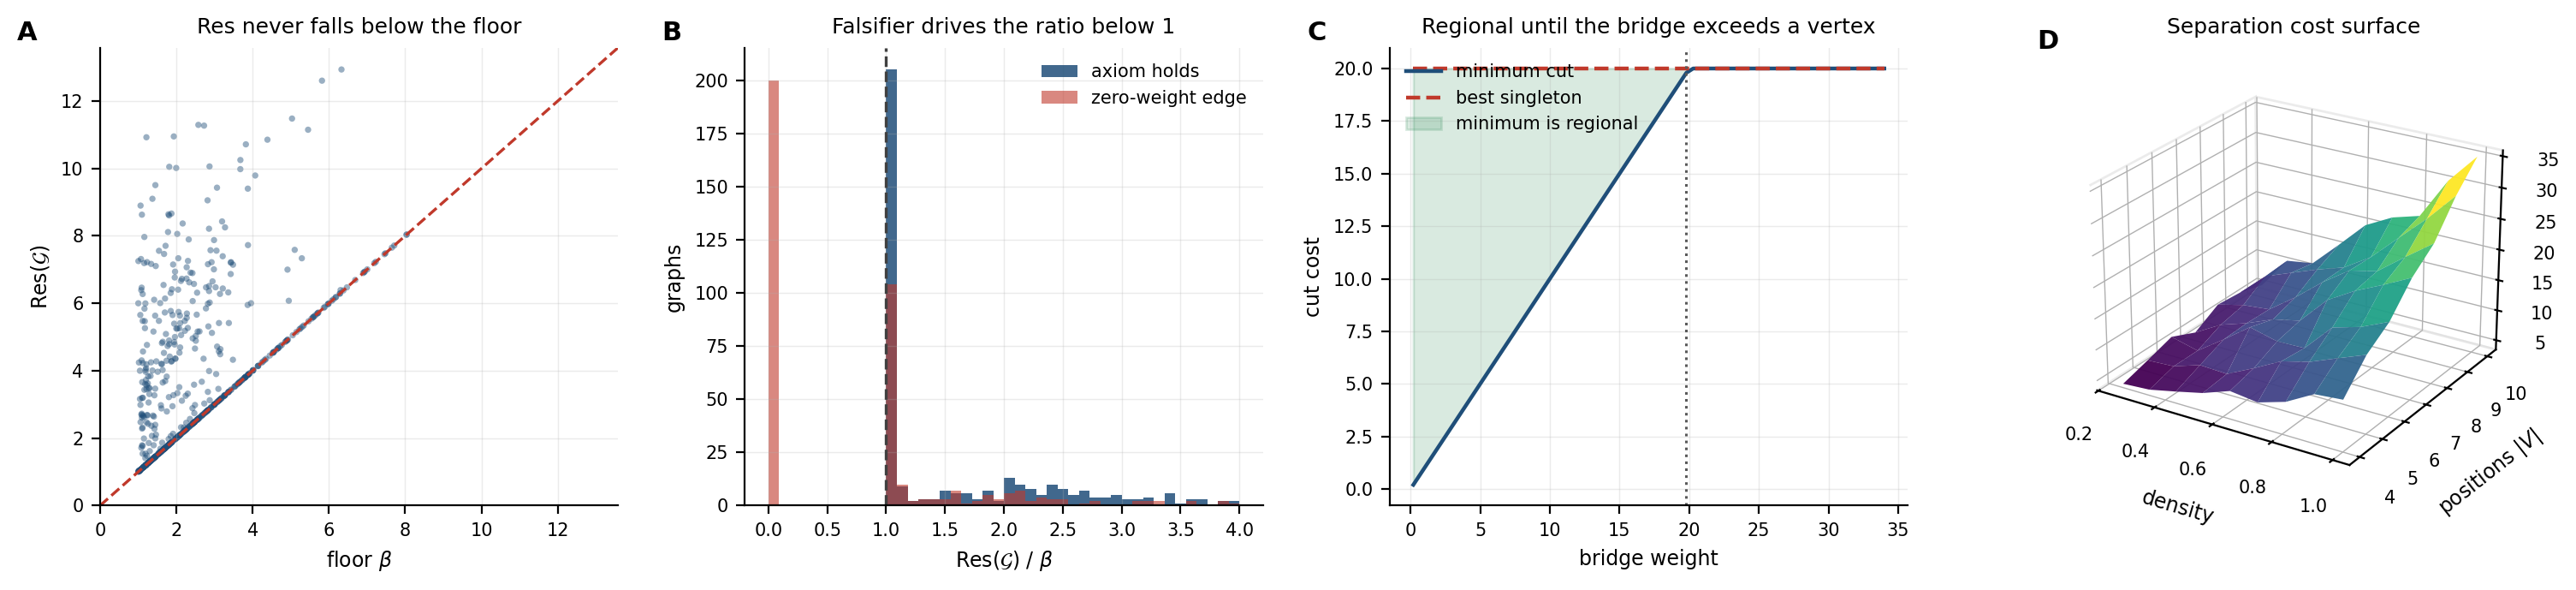
\includegraphics[width=\textwidth]{figures/panel_1}
    \caption{\textbf{Separation is bounded away from zero, and the bound is
    attained by a region rather than by a position.}
    (\textbf{A})~Separation cost $\Res(\Gph)$ on the linear $y$-axis
    ($1.01$ to $12.9$) versus the floor $\flo$ on the linear $x$-axis
    ($1.00$ to $8.04$), for $600$ randomly generated connected contact graphs
    on three to eight positions; the dashed line is the identity. Every point
    lies on or above it, so no graph separates a nonempty proper part from its
    complement more cheaply than its least edge weight. Points on the line are
    graphs whose minimum cut is a single cheapest edge; points above it are
    graphs in which every separation severs more
    (\Cref{thm:floor}).
    (\textbf{B})~Distribution of the ratio $\Res(\Gph)/\flo$ on the linear
    $x$-axis ($0$ to $4$) over $400$ graphs, with \Cref{ax:costly} holding
    (dark) and with one edge weight set to zero (light); the dashed line marks
    unity. The intact series lies entirely at or above $1$; the falsified
    series places $109$ of $200$ graphs at $0$. The bound is therefore a
    consequence of the axiom and not of the definition, since removing the
    axiom removes the bound.
    (\textbf{C})~Cut cost on the linear $y$-axis ($0$ to $20$) versus the
    weight of the joining edge on the linear $x$-axis ($0.2$ to $34$), for the
    two-triangle witness of \Cref{thm:regional} with all six internal weights
    fixed at $10$. The minimum cut (solid) rises with the bridge while the
    best singleton cut (dashed) is constant at $20$; the shaded interval is
    where the minimum is attained by a three-position region and by no
    singleton, and the dotted line marks the crossover at bridge weight $20$
    beyond which the two coincide. Individuation has extent
    (\Cref{cor:no-point}).
    (\textbf{D})~Three-dimensional surface of mean separation cost on the
    $z$-axis ($4.08$ to $35.3$) over edge density on the $x$-axis ($0.25$ to
    $1.0$) and position count $|\V|$ on the $y$-axis ($4$ to $10$), each cell
    the mean of $14$ graphs. The surface is strictly positive at every
    combination and rises with both parameters; there is no direction in the
    parameter space along which separation cost approaches zero, which is the
    absence of the limiting process that \Cref{rem:floor-content} identifies
    as the theorem's content. Viewing angle: elevation $24^{\circ}$, azimuth
    $-58^{\circ}$.}
    \label{fig:panel1}
\end{figure*}

\begin{figure*}[!htbp]
    \centering
    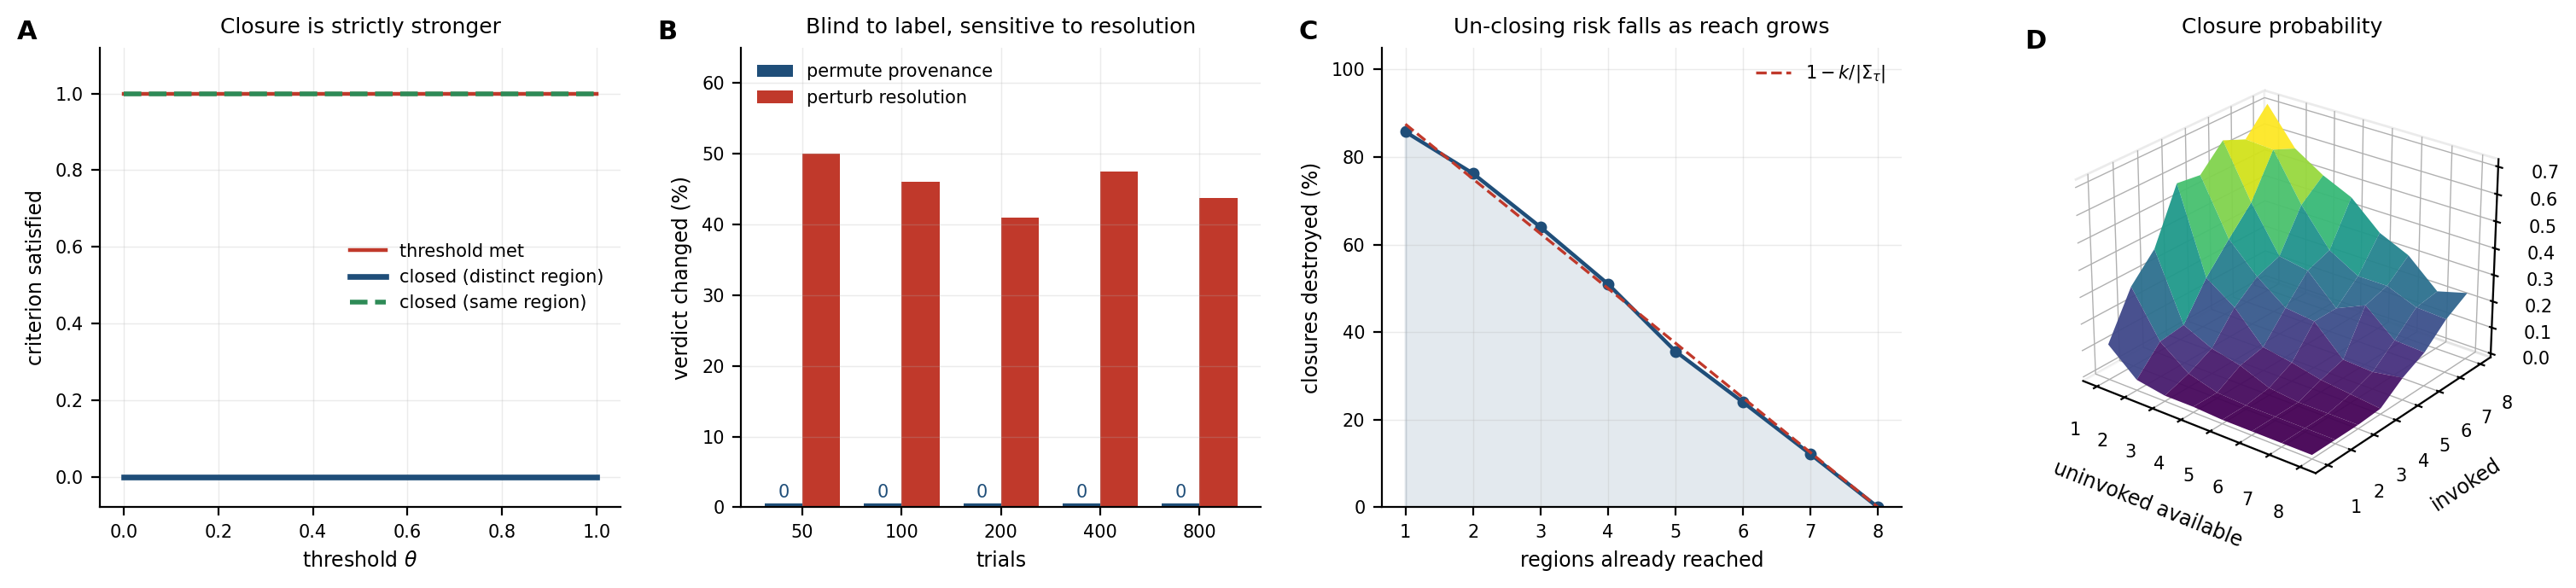
\includegraphics[width=\textwidth]{figures/panel_2}
    \caption{\textbf{Closure is not a threshold, does not read provenance, and
    is not monotone in what is available.}
    (\textbf{A})~Criterion satisfied, on the binary $y$-axis, versus the
    confidence threshold $\theta$ on the linear $x$-axis ($0$ to $1$), on the
    witness of \Cref{thm:closure-stronger}: two disjoint triangles joined by a
    single edge, with both considerations carrying confidence $1$. The
    threshold criterion (upper trace) is met at every $\theta$; the closure
    criterion (lower trace) fails at every $\theta$, because the uninvoked
    consideration resolves into the second triangle. Replacing that
    consideration by one resolving into the \emph{first} triangle restores
    closure at every $\theta$ (dashed, coincident with the upper trace),
    locating the failure in the distinct region rather than in the form of
    \Cref{def:closure}. No adjustment of $\theta$ converts one criterion into
    the other.
    (\textbf{B})~Percentage of verdicts changed on the linear $y$-axis versus
    the number of randomised configurations on the categorical $x$-axis ($50$
    to $800$). Permuting provenance labels changes the verdict in exactly
    zero cases at every sample size (dark, annotated, drawn as a rule at the
    axis since the bars have no height); perturbing \emph{resolutions} with
    the same machinery changes it in $41.0$ to $50.0$ per cent of cases
    (light). It is the asymmetry between the two counts, not the invariance
    alone, that distinguishes \Cref{thm:blind} from a definition too coarse to
    register anything: a definition insensitive to everything would have
    produced invariance under both perturbations.
    (\textbf{C})~Percentage of existing closures destroyed by adjoining one
    further available consideration, on the linear $y$-axis ($0$ to $85.8$),
    versus the number of regions the invoked set already reaches, on the
    linear $x$-axis ($1$ to $8$), drawn from a pool of eight distinct regions;
    the dashed line is the analytic prediction $1-k/|\Sig_\tau|$. The measured
    curve tracks it across the range and reaches zero exactly when the invoked
    reach exhausts the pool. A commitment can therefore lapse because
    something new became available, with no agent having changed its mind
    about anything already considered (\Cref{rem:not-mono-avail}).
    (\textbf{D})~Three-dimensional surface of the probability that a search is
    closed, on the $z$-axis ($0$ to $0.713$), over the number of uninvoked
    available considerations on the $x$-axis ($1$ to $8$) and the number
    invoked on the $y$-axis ($1$ to $8$), each cell $160$ draws from a
    six-region pool. The surface falls steeply along the availability axis and
    rises along the invoked axis: closure is a joint condition on both, and in
    particular is not a property of the evidence in hand
    (\Cref{prop:mono-invoked}). Viewing angle: elevation $26^{\circ}$, azimuth
    $-52^{\circ}$.}
    \label{fig:panel2}
\end{figure*}

\begin{figure*}[!htbp]
    \centering
    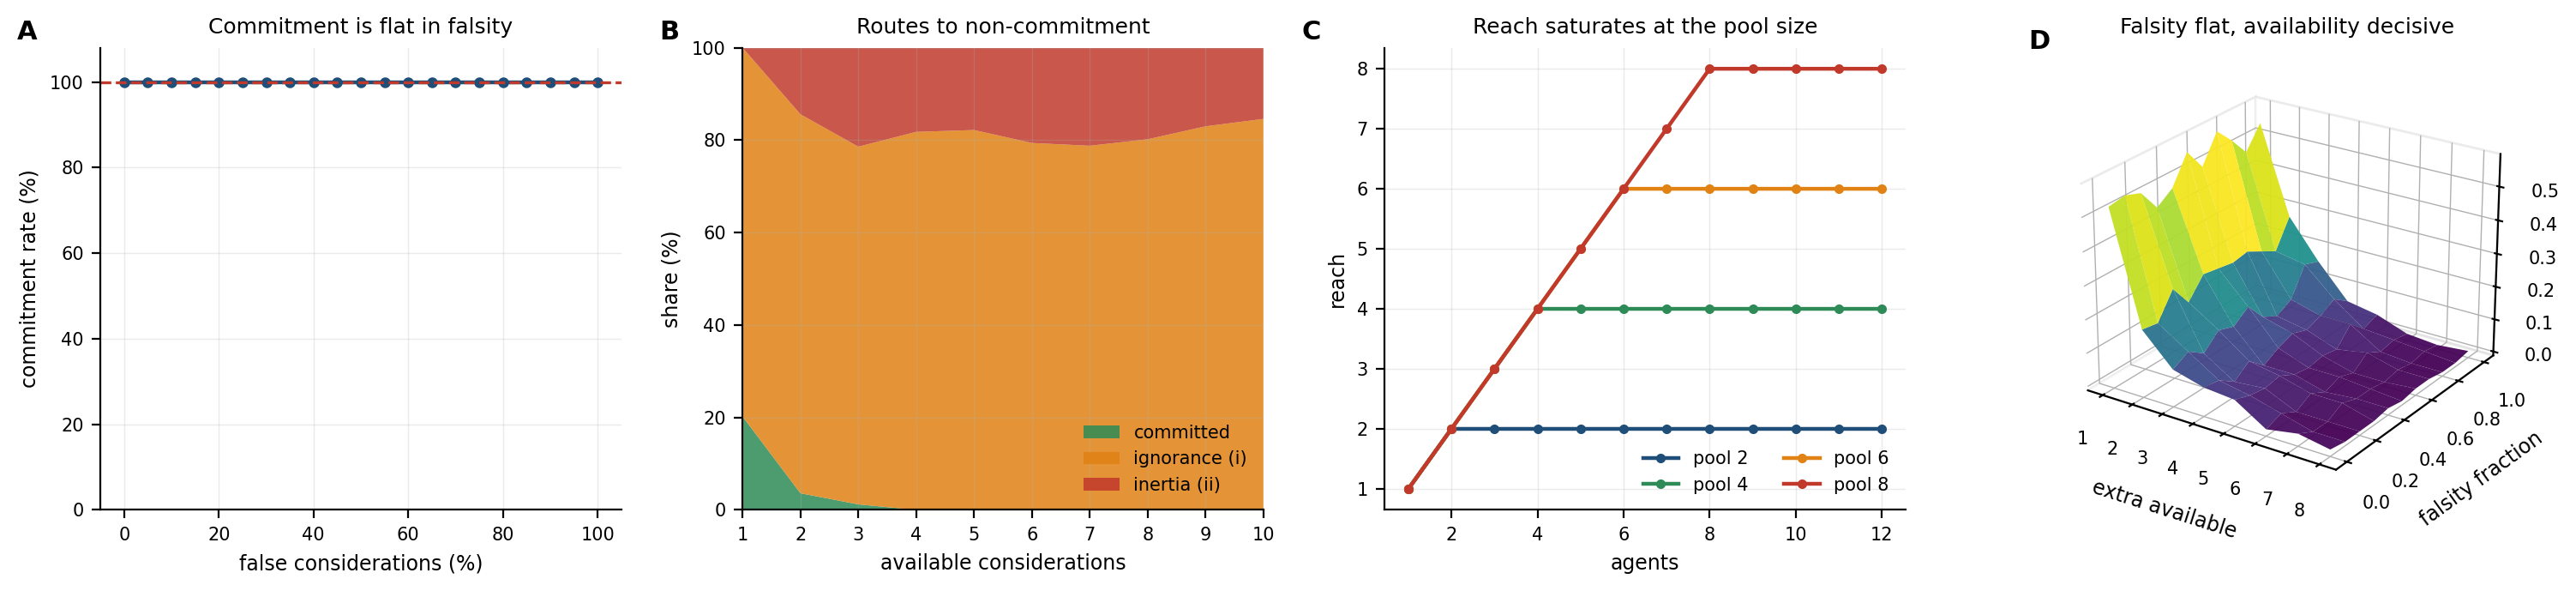
\includegraphics[width=\textwidth]{figures/panel_3}
    \caption{\textbf{Correctness is not a term in the commitment condition,
    and non-commitment decomposes into three structurally distinct routes.}
    (\textbf{A})~Commitment rate on the linear $y$-axis ($0$ to $108$ per
    cent) versus the percentage of considerations that are false on the linear
    $x$-axis ($0$ to $100$), holding resolutions fixed, $500$ configurations
    per point; the dashed line marks $100$ per cent. The measured rate is
    exactly $100$ per cent at every level of falsity including the endpoint at
    which \emph{every} consideration is false. Commitment is therefore
    invariant under substitution of false considerations for true ones with
    the same resolution (\Cref{thm:truth-blind}). The theorem does not assert
    that falsity is harmless: a population committed to the wrong region
    encounters the consequences of being there, but by the ordinary route of
    occupying an unsuitable region rather than through any failure of the
    mechanism (\Cref{rem:truth-scope}).
    (\textbf{B})~Share of outcomes on the linear $y$-axis ($0$ to $100$ per
    cent) versus the number of available considerations on the linear $x$-axis
    ($1$ to $10$), $500$ configurations per point, stacked by the
    classification of \Cref{prop:three-routes}. Commitment falls from $20.2$
    per cent at a single available consideration to below $1$ per cent by
    four; ignorance --- no invoked consideration reaches the target ---
    dominates throughout at $77$ to $82$ per cent; inertia --- the target is
    reached but closure fails --- grows as the available set does. The three
    are distinguished by different tests, which is why they present
    differently from the inside (\Cref{rem:three-feel}).
    (\textbf{C})~Reach on the linear $y$-axis ($1$ to $8$) versus population
    on the linear $x$-axis ($1$ to $12$), for pools of two, four, six and
    eight distinct resolutions. Each series grows one-for-one until the pool
    is exhausted and is exactly flat thereafter. Reach is bounded by the
    number of \emph{distinct} resolutions and not by headcount, and the
    ceiling $|\Sig_\tau(\Gph)|$ counts regions the graph possesses, so no
    recruitment raises it (\Cref{prop:ceiling,rem:heterogeneity}).
    (\textbf{D})~Three-dimensional surface of commitment probability on the
    $z$-axis ($0$ to $0.583$) over the number of extra available
    considerations on the $x$-axis ($1$ to $8$) and the falsity fraction on
    the $y$-axis ($0$ to $1$), $120$ draws per cell. The surface is flat along
    the falsity axis and falls sharply along the availability axis, exhibiting
    \Cref{thm:truth-blind} and \Cref{rem:not-mono-avail} on one pair of
    coordinates: what an agent believes wrongly does not move the verdict, and
    what it has not yet considered does. Viewing angle: elevation
    $24^{\circ}$, azimuth $-56^{\circ}$.}
    \label{fig:panel3}
\end{figure*}

\begin{figure*}[!htbp]
    \centering
    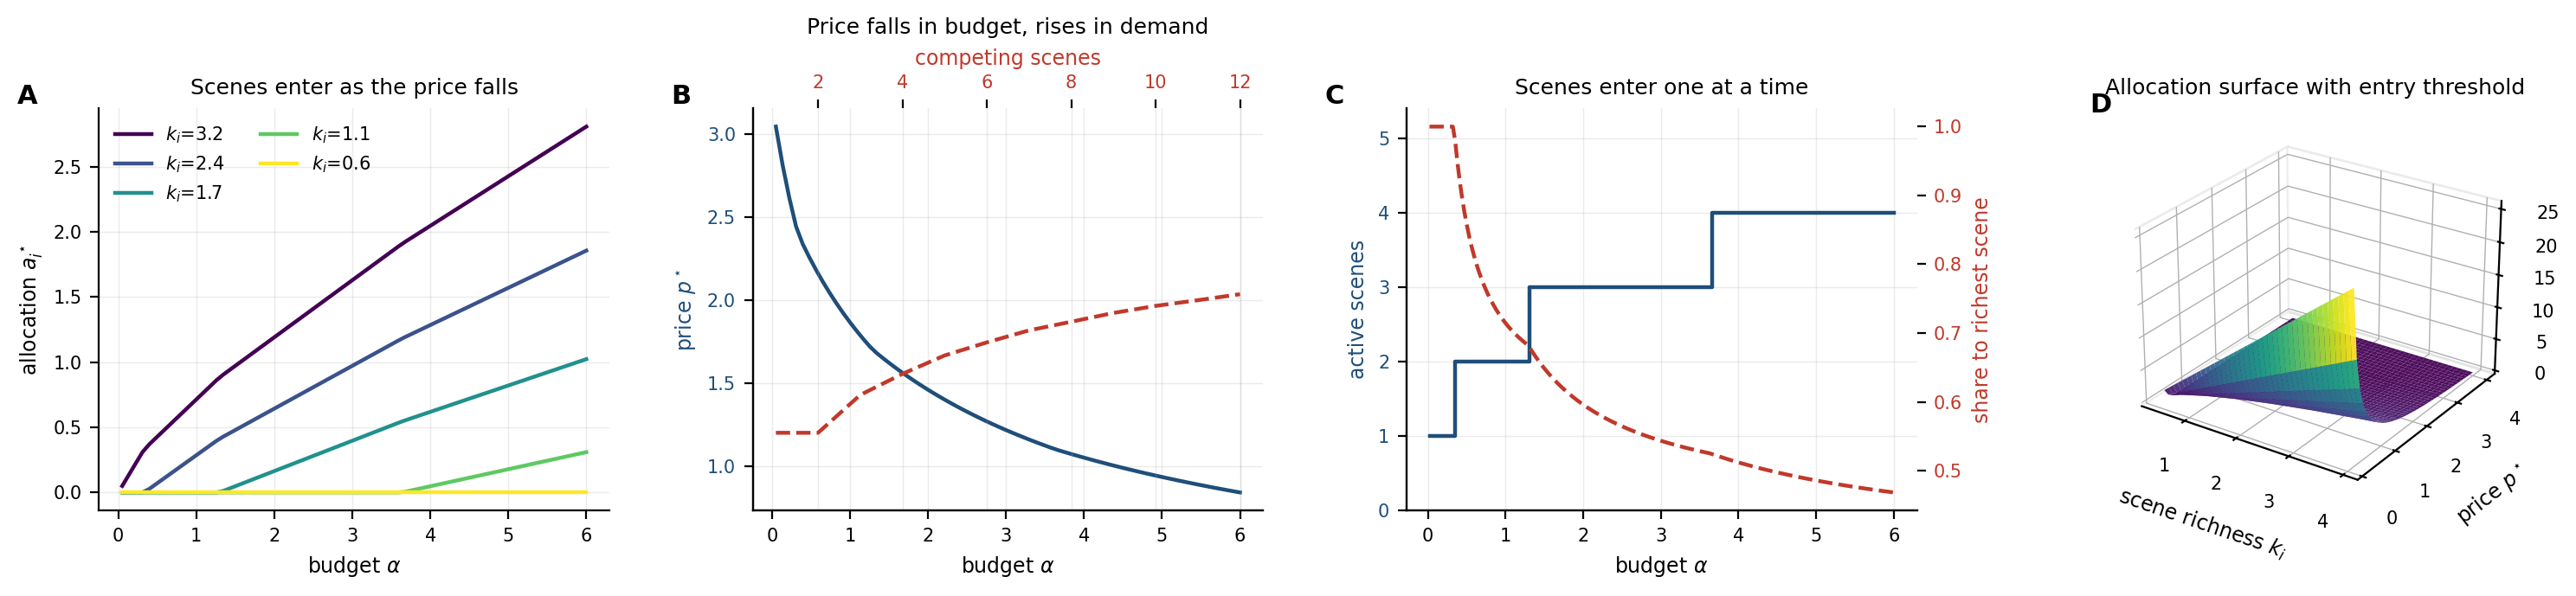
\includegraphics[width=\textwidth]{figures/panel_4}
    \caption{\textbf{A bounded capacity divides across concurrent demands by
    water-filling at a single price, with scenes entering at their own
    thresholds.}
    (\textbf{A})~Optimal allocation $a_i^{\star}$ on the linear $y$-axis ($0$
    to $2.81$) versus the budget $\att$ on the linear $x$-axis ($0.05$ to
    $6$), for five scenes with gain profiles $\gamma_i(a)=k_i\log(1+a)$ and
    richness $k_i\in\{3.2,2.4,1.7,1.1,0.6\}$. Each curve leaves zero at its
    own entry threshold --- the budget at which the price falls to
    $\gamma_i'(0)=k_i$ --- and the poorest scene remains unattended over the
    entire range plotted. Just above its threshold a scene receives a positive
    but arbitrarily small allocation, which is the formal minimal
    acknowledgement of \Cref{cor:token}.
    (\textbf{B})~Attention price $\price$ on the linear $y$-axis ($0.84$ to
    $3.05$) versus the budget on the lower linear $x$-axis ($0.05$ to $6$,
    solid) and versus the number of competing scenes on the upper linear
    $x$-axis ($1$ to $12$, dashed, $\price$ from $1.20$ to $2.04$). The price
    is monotone decreasing in capacity and monotone increasing in demand,
    both as \Cref{thm:waterfill} requires of the multiplier of a binding
    budget constraint.
    (\textbf{C})~Number of attended scenes on the left linear $y$-axis ($0$ to
    $5$, step) and the share of capacity received by the richest scene on the
    right linear $y$-axis ($0.5$ to $1.0$, dashed), versus the budget on the
    linear $x$-axis ($0.02$ to $6$). Scenes are taken up one at a time as the
    price crosses successive thresholds, while the richest scene's share falls
    monotonically from unity: the agent becomes thinly present in several
    contexts rather than fully present in one. This is the derived content of
    \Cref{cor:preoccupied}, and it is the one result in the figure conditional
    on the environmental assumption \Cref{ax:concave}; under increasing
    returns the optimum is concentration instead (\Cref{rem:nonconcave}).
    (\textbf{D})~Three-dimensional surface of the allocation
    $(\gamma_i')^{-1}(\price)=k_i/\price-1$ on the $z$-axis ($0$ to $25$) over
    scene richness $k_i$ on the $x$-axis ($0.4$ to $4.0$) and price $\price$
    on the $y$-axis ($0.15$ to $4.0$), clipped at zero where $k_i\le\price$.
    The ridge along which the surface leaves the zero plane is the entry
    threshold, and the divergence at small price is the regime in which an
    idle agent is forthcoming everywhere at once. Viewing angle: elevation
    $26^{\circ}$, azimuth $-56^{\circ}$.}
    \label{fig:panel4}
\end{figure*}

\begin{figure*}[!htbp]
    \centering
    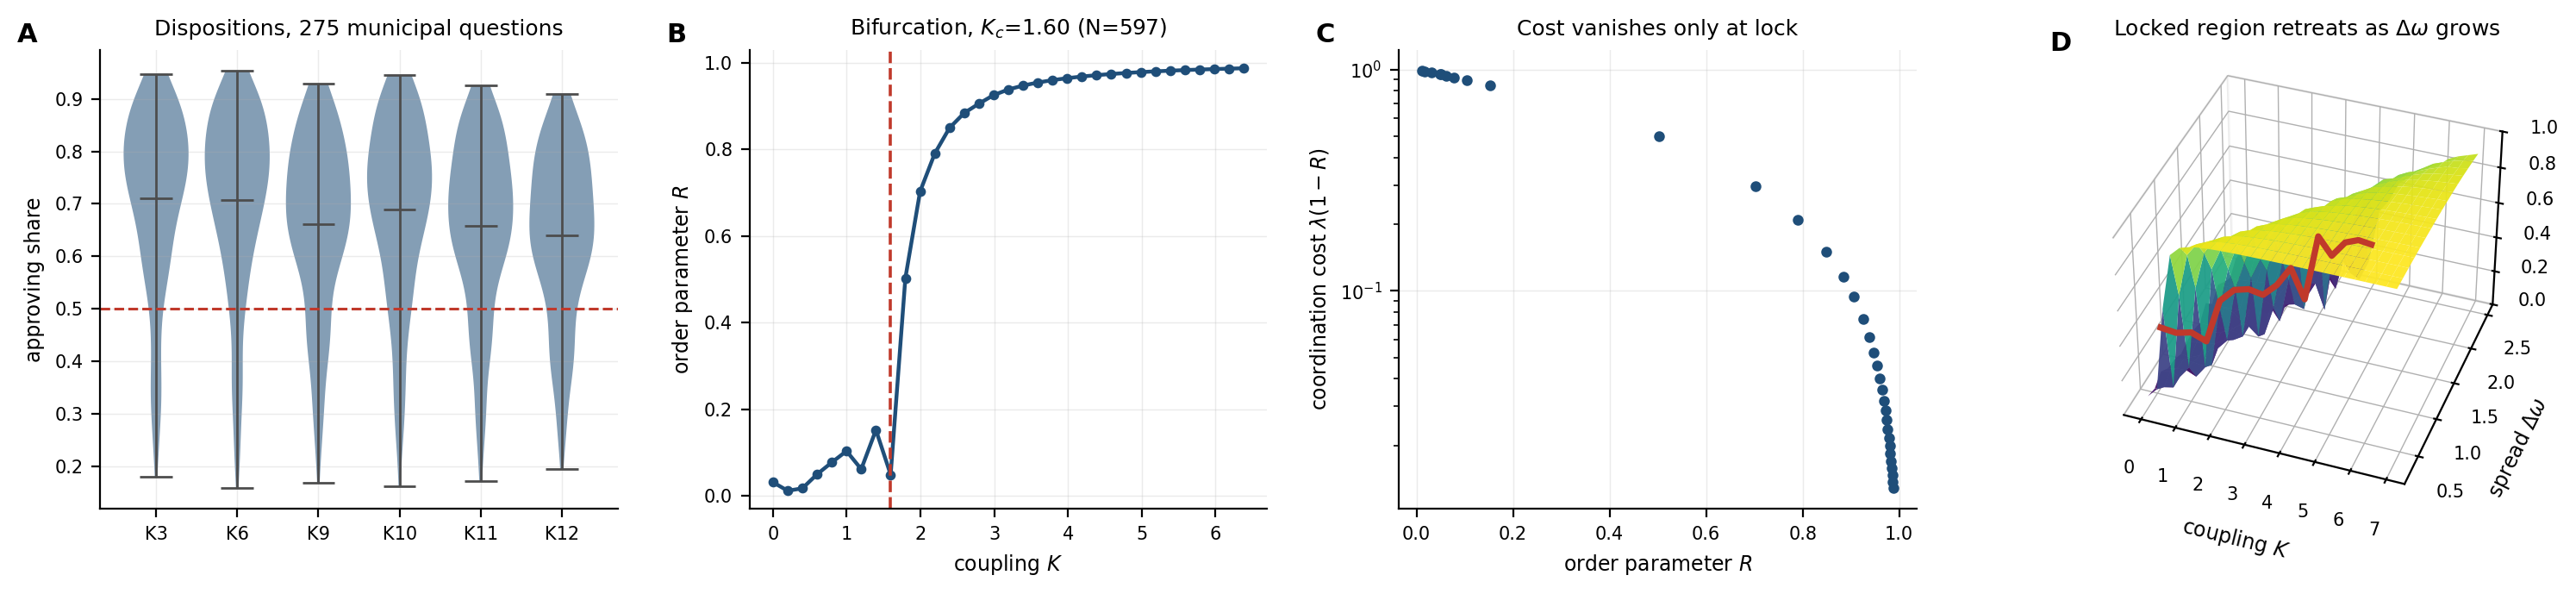
\includegraphics[width=\textwidth]{figures/panel_5}
    \caption{\textbf{The synchronisation threshold, measured on the
    heterogeneity of the Z\"urich record.}
    (\textbf{A})~Approving share on the linear $y$-axis ($0.158$ to $0.954$)
    for each of the six consistently reported municipal units on the
    categorical $x$-axis, as violin densities over all $275$ city questions of
    2002--2026 \citep{ssz_abstimmungen}; the dashed line marks the $0.5$
    majority. The dispersion between units, not their central tendency, is the
    velocity spread $\Delta\omega$ that fixes the threshold in the remaining
    charts, so the parameter is measured from the record rather than assumed.
    (\textbf{B})~Order parameter $\Ord$ on the linear $y$-axis ($0.012$ to
    $0.987$) versus coupling $K$ on the linear $x$-axis ($0$ to $6.38$), with
    each unit treated as a tempo class populated in proportion to its resident
    count, giving $N=597$ oscillators, integrated $3000$ steps at $dt=0.05$;
    the dashed line is the predicted critical coupling $\Kc=1.60$. Below it
    the order parameter remains at or under $0.107$ and does not drift upward
    under continued integration; above $2\Kc$ it exceeds $0.951$. The
    populating step is necessary rather than cosmetic: \Cref{thm:kuramoto}(ii)
    is a mean-field statement and six oscillators alone leave the transition
    buried in finite-size fluctuation.
    (\textbf{C})~Coordination cost $\lambda_c(1-\Ord)$ on the logarithmic
    $y$-axis ($0.0128$ to $0.988$) versus the order parameter on the linear
    $x$-axis ($0$ to $1$), evaluated on the achieved $\Ord$ of chart~B. The
    cost falls by nearly two decades only as $\Ord$ approaches unity and
    vanishes exactly at lock, which is the equality case of
    \Cref{thm:phaselock}; away from lock it is strictly positive.
    (\textbf{D})~Three-dimensional surface of the order parameter on the
    $z$-axis ($0$ to $1$) over coupling $K$ on the $x$-axis ($0$ to $7$) and
    velocity spread $\Delta\omega$ on the $y$-axis ($0.3$ to $2.5$), computed
    on one fixed standardised velocity sample of $400$ oscillators rescaled
    per row so that rows differ only in spread and not in sampling noise; the
    solid line is the predicted $\Kc=2\sigma_\omega\sqrt{2\pi}/\pi$ lifted onto
    the surface. The locked plateau retreats toward larger $K$ as
    heterogeneity grows, and the predicted threshold tracks the boundary. The
    residual roughness below the threshold is genuine finite-size fluctuation
    of $\Ord$ in the incoherent regime, not numerical noise, and is left
    unsmoothed. Viewing angle: elevation $38^{\circ}$, azimuth $-70^{\circ}$.}
    \label{fig:panel5}
\end{figure*}

\begin{figure*}[!htbp]
    \centering
    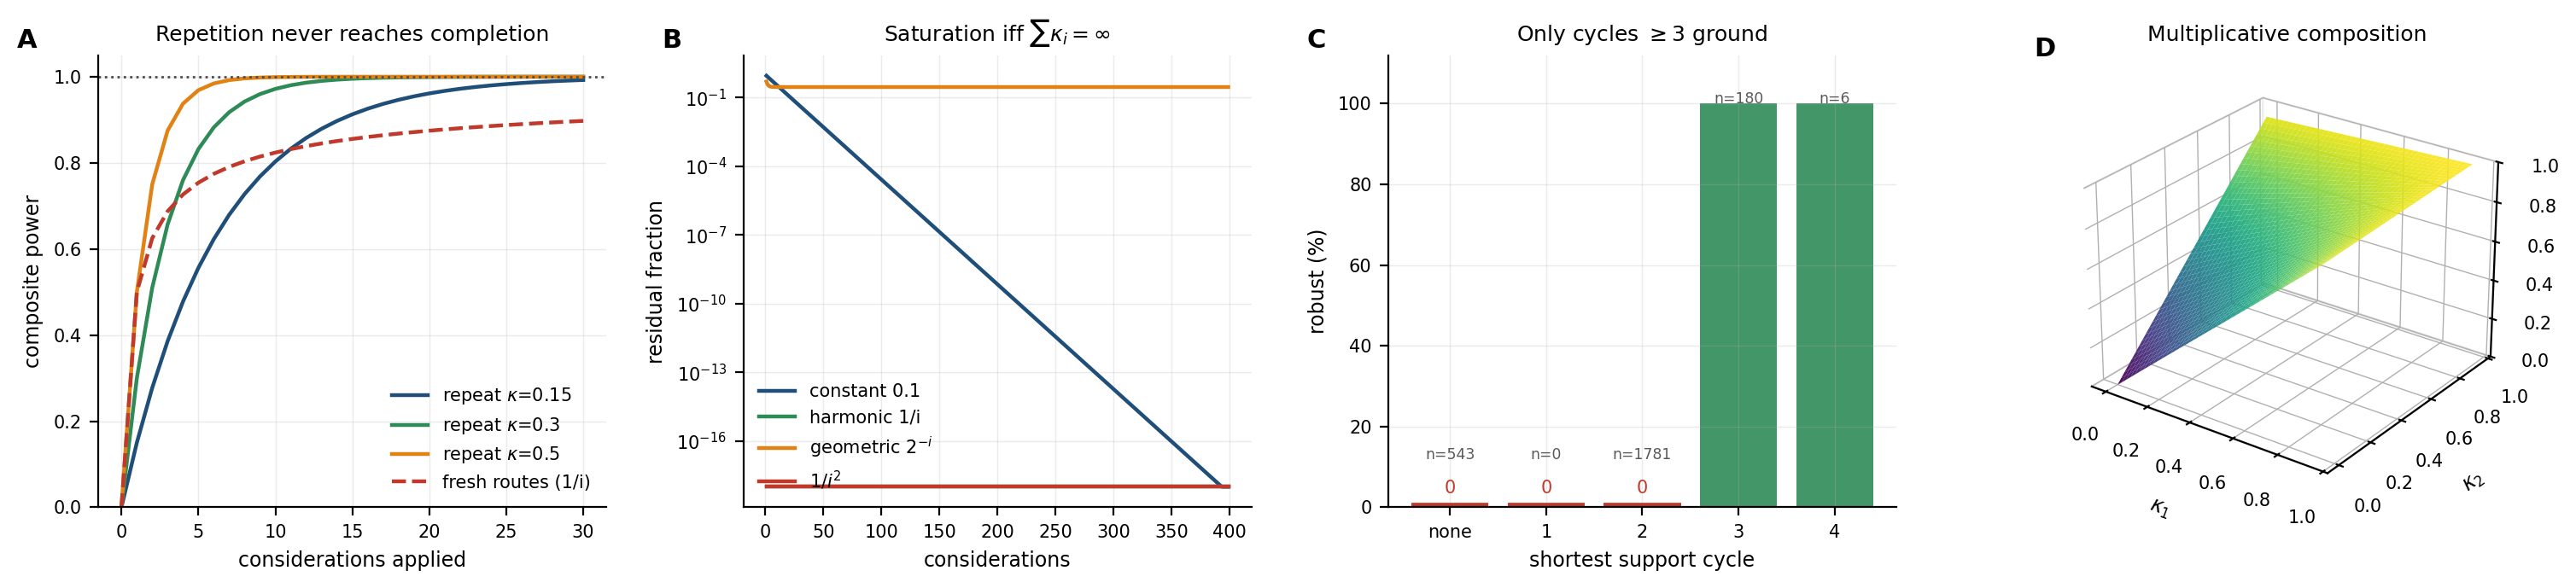
\includegraphics[width=\textwidth]{figures/panel_6}
    \caption{\textbf{Considerations compose multiplicatively, repetition
    saturates strictly below completion, and grounding requires a support
    cycle of length at least three.}
    (\textbf{A})~Composite power on the linear $y$-axis ($0$ to $1$) versus
    the number of considerations applied on the linear $x$-axis ($0$ to $30$),
    for a single consideration of power $\kappa\in\{0.15,0.30,0.50\}$ repeated
    (solid) and for a sequence of fresh routes with powers $0.5/i$ (dashed,
    reaching $0.897$ at $30$); the dotted line marks unity. Every repetition
    series increases, converges toward unity and attains it at no finite
    count, with strictly decaying increments
    (\Cref{cor:diminishing,cor:saturate}).
    (\textbf{B})~Residual fraction $\prod_i(1-\kappa_i)$ on the logarithmic
    $y$-axis ($10^{-18}$ to $1$) versus the number of considerations on the
    linear $x$-axis ($1$ to $399$), for four power sequences. The
    divergent-sum sequences (constant $0.1$; harmonic $1/i$) drive the
    residual toward zero; the convergent-sum sequences (geometric $2^{-i}$;
    inverse-square $1/i^{2}$) plateau at a positive constant and remain there.
    This is the dichotomy of \Cref{thm:saturation} and the structural
    condition on a long campaign: a proposal whose reachable considerations
    have summable powers is never closed by persistence
    (\Cref{rem:campaign}).
    (\textbf{C})~Percentage of support structures that are robust on the
    linear $y$-axis ($0$ to $100$) by shortest directed cycle length on the
    categorical $x$-axis, exhaustively over four-position digraphs with at
    most six edges, with the number of structures in each class annotated.
    Acyclic structures and cycles of length one and two are robust in no case
    and are drawn as rules at the axis with their zero marked; every structure
    whose shortest cycle has length three or four is robust without exception.
    Two elements can only assert each other; three can check each other
    (\Cref{thm:linear,thm:three}), and a repeated single item is a one-cycle
    and therefore grounds nothing (\Cref{cor:repeat-nothing}).
    (\textbf{D})~Three-dimensional surface of the composite power
    $1-(1-\kappa_1)(1-\kappa_2)$ on the $z$-axis ($0$ to $1$) over the two
    constituent powers on the $x$- and $y$-axes ($0$ to $0.95$). The sheet
    rises toward but never attains unity, and its curvature is the diminishing
    return each additional consideration closes of the remaining above-floor
    distance (\Cref{thm:multiplicative}). Viewing angle: elevation
    $26^{\circ}$, azimuth $-54^{\circ}$.}
    \label{fig:panel6}
\end{figure*}

\begin{figure*}[!htbp]
    \centering
    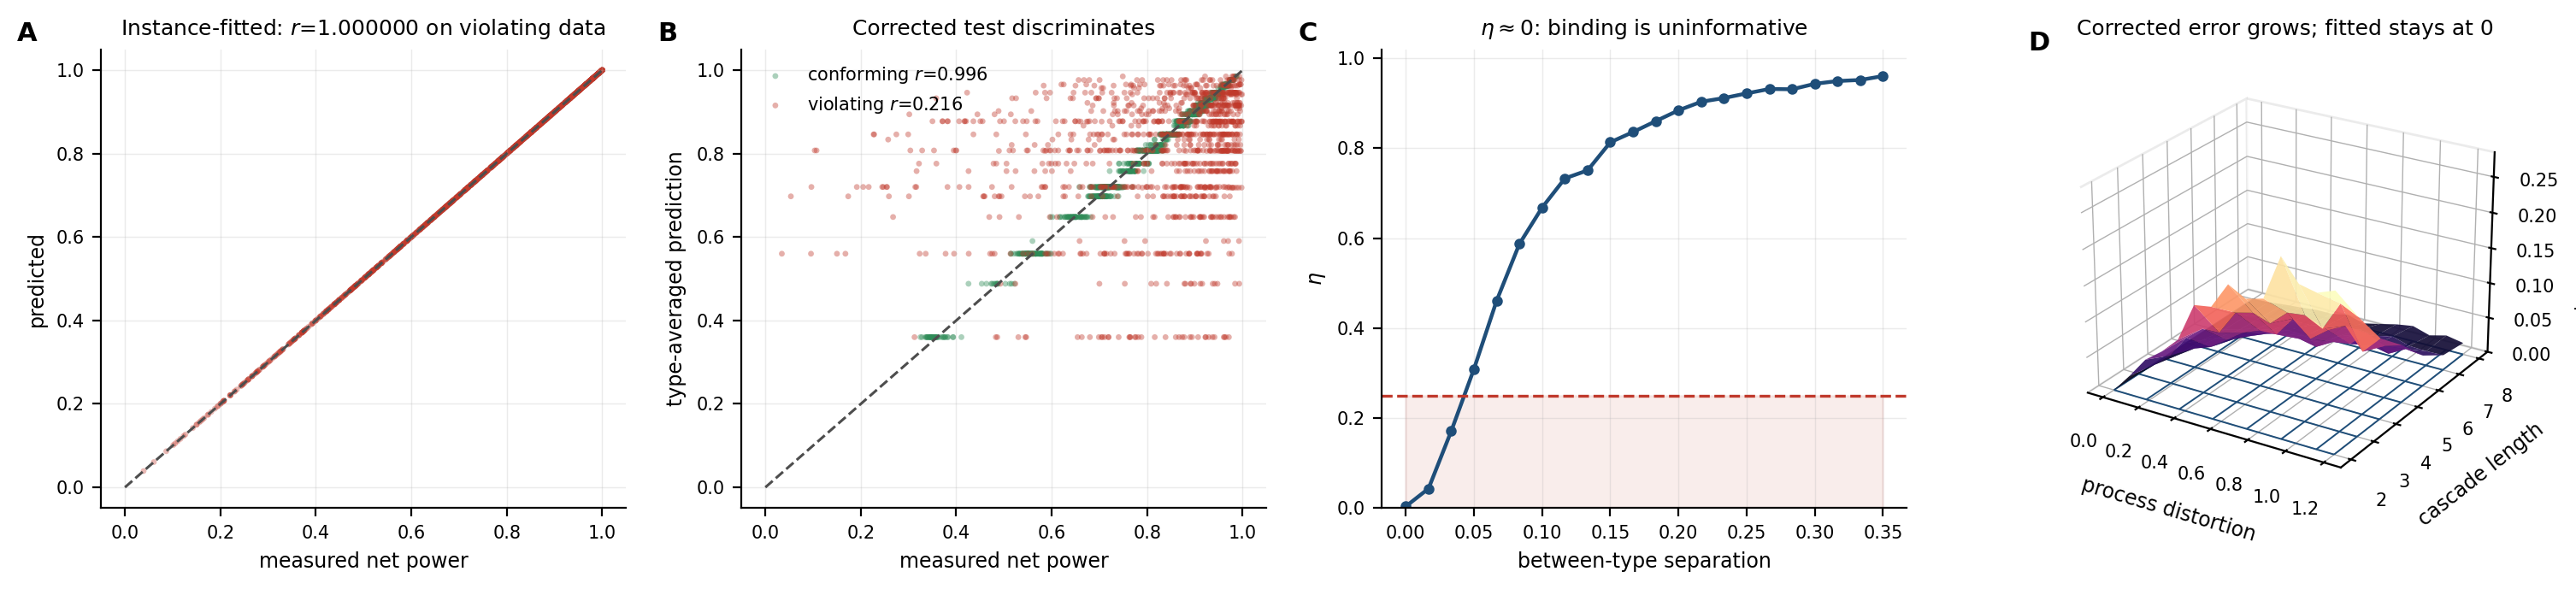
\includegraphics[width=\textwidth]{figures/panel_7}
    \caption{\textbf{The natural test of the composition law has no null; the
    type-averaged test does; and the diagnostic says when even it has no
    power.}
    (\textbf{A})~Instance-specific prediction $1-\prod_i(1-\kappa_i)$ on the
    linear $y$-axis ($0$ to $1$) versus the measured net power
    $(S_1-S_{n+1})/(S_1-\flo)$ on the linear $x$-axis ($0$ to $1$), for
    $1500$ cascades of length two to six generated by a process that violates
    \Cref{thm:multiplicative} by construction, each step's reduction being
    scaled by an arbitrary distortion factor. The points lie on the diagonal
    (dashed) with Pearson $r=1.000000$: under instance-specific estimation the
    two quantities are the \emph{same algebraic expression}, so the statistic
    attains its degenerate value on every data set whatsoever, including data
    generated by a process violating the law it purports to confirm. The test
    cannot fail and therefore has no power against any alternative
    (\Cref{thm:telescoping,cor:no-null}).
    (\textbf{B})~The same comparison under type-averaged estimation, in which
    the constituent powers are the means of their event types computed
    excluding the predicted cascade. Conforming data attain $r=0.996$ and
    data violating the composition law fall to $r=0.216$, with the violating
    cloud departing visibly from the diagonal. Breaking the dependence of the
    prediction on the predicted cascade's own observations restores a null
    (\Cref{thm:typeavg}).
    (\textbf{C})~Separation diagnostic $\eta=\Var_{\mathrm{b}}/
    (\Var_{\mathrm{b}}+\Var_{\mathrm{w}})$ on the linear $y$-axis ($0.004$ to
    $0.961$) versus the imposed between-type separation on the linear $x$-axis
    ($0$ to $0.35$), at fixed within-type dispersion; the shaded band below
    the dashed line at $0.25$ is the regime in which per-type means are
    indistinguishable. There, predictions are constant at fixed cascade length
    and no comparison among composition rules can be separated, so a negative
    result is evidence about the observable rather than about the process
    (\Cref{prop:uninformative}).
    (\textbf{D})~Three-dimensional mean absolute prediction error on the
    $z$-axis over process distortion on the $x$-axis ($0$ to $1.2$) and
    cascade length on the $y$-axis ($2$ to $8$), $60$ cascades per cell, for
    the type-averaged test (surface, rising to $0.247$) and the
    instance-specific test (wireframe, bounded by $5.7\times10^{-17}$ across
    the whole grid). The corrected error grows with distortion while the
    fitted error is pinned at floating-point zero for every process: the
    obstruction and its remedy in one view. Viewing angle: elevation
    $24^{\circ}$, azimuth $-58^{\circ}$.}
    \label{fig:panel7}
\end{figure*}

\begin{figure*}[!htbp]
    \centering
    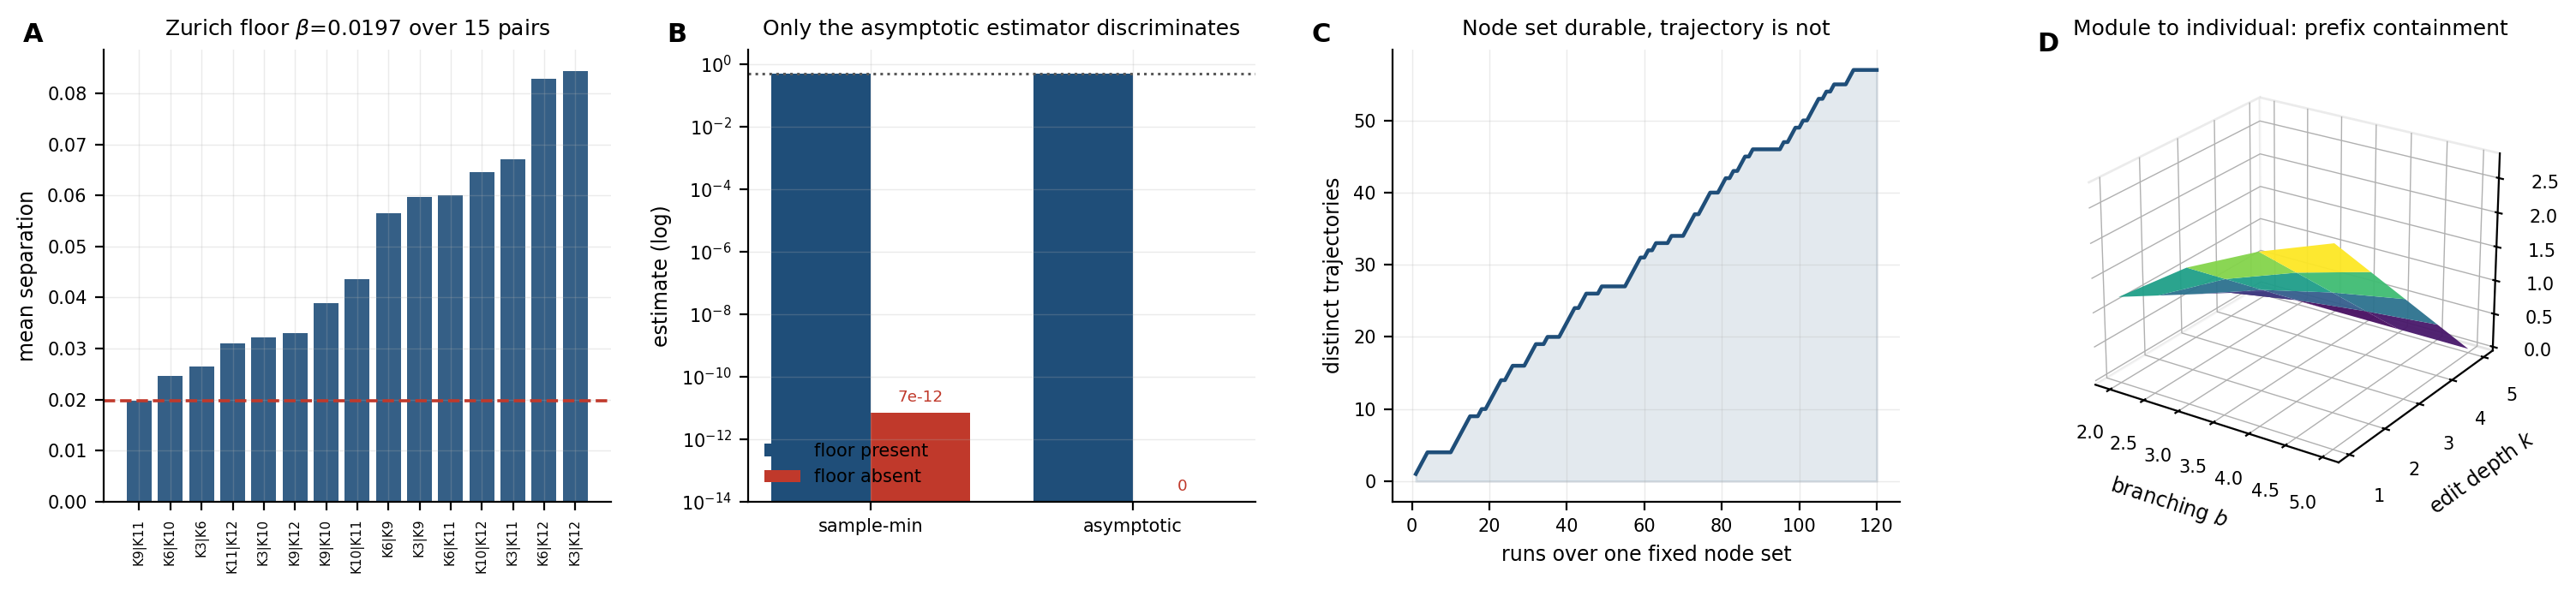
\includegraphics[width=\textwidth]{figures/panel_8}
    \caption{\textbf{The measured floor of the Z\"urich binding, the two
    discharges of the floor obligation, and the runtime's two durabilities.}
    (\textbf{A})~Mean separation on the linear $y$-axis ($0.0197$ to $0.0844$)
    for each of the $15$ receiver pairs on the categorical $x$-axis, sorted
    ascending, computed as the mean absolute difference of approving shares
    over all $275$ questions; the dashed line marks the least pair separation,
    which is the measured floor $\flo=0.0197$. It is strictly positive: even
    the two most similar units differ by about two percentage points on
    average across the record, so the floor is measured rather than assumed.
    Published shares are rounded to $0.1$ percentage points and two units
    therefore coincide exactly on $30$ of $4125$ single questions
    ($0.73$ per cent); a floor defined per question would be zero for a
    reason having nothing to do with the polity, which is why obligation (S4)
    is discharged on receiver \emph{pairs} over the whole record, as
    \Cref{def:cut} requires.
    (\textbf{B})~Floor estimate on the logarithmic $y$-axis ($10^{-14}$ to
    $3$) for the two discharges on the categorical $x$-axis, evaluated on a
    synthetic process with a genuine floor at $0.5$ (dark) and on one
    constructed to have no floor (light), $4000$ observations each; the dotted
    line marks the true value $0.5$. The sample-minimum estimator returns
    $0.500$ and $7\times10^{-12}$ --- positive on \emph{both} processes, so a
    positivity claim from it carries no evidential weight; the asymptotic
    estimator returns $0.499$ and exactly $0$, discriminating between them and
    therefore capable of being wrong (\Cref{rem:floor-obligation}).
    (\textbf{C})~Cumulative count of distinct trajectories on the linear
    $y$-axis ($1$ to $57$) versus runs executed on the linear $x$-axis ($1$ to
    $120$), over one fixed six-node set. The node set is durable and can be
    catalogued, frozen and imported; the induced causal edge relation is
    constituted by the run and is not schedulable in advance, so
    reproducibility attaches to the protocol and its provenance rather than to
    the readings (\Cref{thm:emergence,cor:repro,rem:repro-meaning}).
    (\textbf{D})~Three-dimensional surface of the blast radius $b^{D-k}$ on
    the logarithmic $z$-axis ($10^{0}$ to $10^{2.6}$) over branching factor
    $b$ on the $x$-axis ($2$ to $5$) and edit depth $k$ on the $y$-axis ($1$
    to $5$), at fixed tree depth $D=5$. An edit at depth $k$ touches exactly
    the leaves beneath its length-$k$ prefix and nothing else, falling from an
    entire imported subtree to a single leaf. A module is a short prefix and
    an individual a full-depth address in one space, so producing an
    individual by pruning is descent in that space rather than a change of
    kind (\Cref{prop:prefix,cor:two-depths}). Viewing angle: elevation
    $24^{\circ}$, azimuth $-56^{\circ}$.}
    \label{fig:panel8}
\end{figure*}


\subsection{Reproducibility}

The prototype is implemented in Python with NumPy and SciPy
\citep{harris2020array,virtanen2020scipy} and graph routines from NetworkX
\citep{hagberg2008exploring}; it is deterministically seeded and persists
every experiment as a JSON record. Reproduction:
\begin{verbatim}
python prototype/runtime.py            # runtime self-test
python validation/run_validation.py    # full suite -> validation/results/
\end{verbatim}
Per \Cref{cor:repro} what is reproduced is the protocol and its provenance;
per \Cref{cor:no-staleness} repeated \emph{sessions} need not agree, and
their differences are data.

% =====================================================================
\part*{Part V --- Scope}
\addcontentsline{toc}{part}{Part V --- Scope}
% =====================================================================

\section{Ethical commitments}
\label{sec:ethics}

The instrument generates agents from public records and places human
participants in extended interaction with them. Four commitments follow, and
each is enforced in the implementation.

\emph{Modules are patterns, not persons.} By \Cref{def:module} a module is a
$\tau$-sufficient region --- a class of disposition. No module is derived
from, or intended to represent, an identified individual, and pruning
(\Cref{def:prune}) yields fictional agents consistent with aggregate
statistics. This is not merely a policy: by \Cref{cor:no-point} the object
individuated at any resolution is a region, so a claim to have reconstructed
a person would be a claim the formalism does not support.

\emph{Participants are told what the instrument cannot do.} By
\Cref{cor:no-attribution} the system cannot report which of a participant's
actions mattered. Presenting any readout that appears to do so would
misrepresent the instrument; \Cref{inv:no-verdict} forbids it structurally.

\emph{Deposits are irreversible and disclosed.} By \Cref{thm:history} nothing
a participant does can be withdrawn from an agent's record. Participants
should be informed of this before a session, since it is unusual.

\emph{No claim is made about the real city.} The binding of
\Cref{sec:binding} uses Z{\"u}rich's public record as a source of vocabulary and
heterogeneity. Statements produced by agents are statements about the
simulated population and are not assertions about Z{\"u}rich, its institutions,
or its residents.

\section{Limitations}
\label{sec:limits}

We record what the development does not establish.

\paragraph{The environmental axiom.} \Cref{thm:waterfill} and everything
depending on it hold only under \Cref{ax:concave}, a claim about the world
rather than the agent. Where scenes offer increasing returns the optimum is
concentration, not division (\Cref{rem:nonconcave}). All results of
\Cref{sec:floor,sec:closure,sec:compose} and
\Cref{thm:alternation,thm:history,thm:char,thm:pair} are independent of it.

\paragraph{Availability.} \Cref{def:closure} quantifies over an available set
the theory does not determine (\Cref{rem:availability}). Closure is decidable
given availability and not from the graph alone. The instrument therefore
cannot say whether a population \emph{ought} to be committed to something.

\paragraph{Empirical adequacy.} We do not claim the agents model human
deliberation. The Z{\"u}rich binding supplies realistic heterogeneity, not
validated behaviour, and no experiment reported here compares agent conduct
to human conduct. Establishing or refuting such a correspondence is the
natural next study and would leave every theorem intact, since none asserts
it.

\paragraph{The independence premise.} \Cref{def:coherence-rule} enforces a
\emph{declared} independence relation. The system cannot verify that
considerations are genuinely independent (\Cref{rem:three-typing}), and three
considerations sharing an upstream source satisfy the rule while violating
its intent.

\paragraph{Scale.} \Cref{inv:deposit} requires the graph to grow
monotonically, and \Cref{thm:history} forbids removing committed record.
Compaction consistent with these invariants --- summarising an agent's
structure while preserving $(\Char,\rec)$ --- is not developed here and is
the principal engineering problem at population scale.

\paragraph{Bands and thresholds.} The only genuine transition in the model is
the bifurcation of \Cref{thm:kuramoto}. Any descriptive banding of the order
parameter is a classification cut-off on a continuous variable and carries no
claim of criticality.

\section{Conclusion}
\label{sec:conclusion}

We set out to specify an instrument in which a well-attested but
hard-to-study social fact --- a proposal believed feasible, opposed by no
one, and never adopted, with no participant experiencing a decision --- can
be instantiated and perturbed.

The explanation the formalism supplies is a single structural observation in
two halves. Commitment is \emph{closure}: an agent commits when every
available consideration resolves into a region already reached, a condition
strictly stronger than any confidence threshold
(\Cref{thm:closure-stronger}). And closure is \emph{blind}: the condition
quantifies over resolutions and mentions nothing else, so it is invariant
under relabelling of provenance (\Cref{thm:blind}) and of truth
(\Cref{thm:truth-blind}). The proposal is not rejected; its region never
closes, and a failure of closure is not an event
(\Cref{rem:no-decision}). At population scale the same absence recurs as a
stable sub-threshold state (\Cref{thm:kuramoto}), and in the algebra of
considerations as a residual that plateaus above the floor
(\Cref{thm:saturation}).

The instrument that follows has an unusual measurement surface, and its
refusals are its principal design commitments rather than concessions. It
cannot report success, because the comparison an exit code encodes is not
computable in it (\Cref{thm:no-verdict}). It cannot report which
consideration mattered, because that verdict is a global minimum expressed in
local terms and no store of local content expresses it
(\Cref{thm:attribution}), and because the terminus does not determine the
path (\Cref{thm:opacity}). And the natural test of its own composition law is
an identity with no null (\Cref{thm:telescoping}), so the instrument exposes
only the corrected, type-averaged test together with the diagnostic that says
when even that has no power (\Cref{prop:uninformative}).

What remains is considerable: a complete and interrogable record of what
propagated, ordinal verdicts on the structure of an argument
(\Cref{cor:ordinal}), distributional signatures across a heterogeneous
population, and a protocol whose provenance is reproducible even though its
readings are not (\Cref{rem:repro-meaning}). We regard the combination ---
complete visibility of what happened, principled inability to determine what
mattered --- as the honest measurement surface for this class of phenomenon,
and note that a version of the instrument reporting an effect attribution
would be evidence that the theory it implements is wrong.

\bibliographystyle{plainnat}
\bibliography{references}

\end{document}
